% ISS presentation template
%
% Change history:
% 24.06.2010    Jürgen Ruoff        Initial creation
% 01.07.2010    Patrick Häcker      Generalization
% 02.07.2010    Patrick Häcker      Adjustment
% 15.11.2010    Patrick Häcker      Improvements
% 20.05.2011    Patrick Häcker      Add presentation type
% 06.01.2012	P. Hermannstädter 	Adapted to ISS, small mods
% 15.07.2019 	A. Bartler			Minor fixes, 16:9 aspect ratio added 



% Insert your name here
\newcommand{\presenter}{Zheming Yin}
\newcommand{\presentershort}{Zheming Yin}
\newcommand{\presenteremail}{PRESENTERMAIL} 		% can be accessed using \presenteremail

% Insert presentation title here
\newcommand{\presentationtitle}{Ray tracing channel simulation for millimeter wave indoor localization system}
\newcommand{\shortpresentationtitle}{Ray tracing channel simulation for millimeter wave indoor localization system}

% Insert type of presentation here (or comment line), probably one of:
% Mitarbeitervortrag, Bachelor-Arbeit, Master-Arbeit, Bachelor thesis, Master thesis
\newcommand{\presentationtype}{Research thesis}

% Insert presentation date here
\newcommand{\presentationdate}{18.07.2024}

% Define the language by uncommenting. If there is an error, try deleting temporary files (*.log, ...)
%\newcommand{\lang}{ngerman}
\newcommand{\lang}{english}

% Uncomment the following line, if you want to create handouts (setting to false does not work!)
%\newcommand{\handoutmode}{true}

% Define aspect ratio to  16:9 or 4:3 by uncommenting
%\newcommand{\aspectratio}{43}
\newcommand{\aspectratio}{169}


% Load beamer class using LSS style
% Default \lang to ngerman
\ifx\lang\undefined
	\newcommand{\lang}{english}
\fi

% Set \handout dependant on \handoutmode
\ifx\handoutmode\undefined
	\newcommand{\handout}{}
\else
	\newcommand{\handout}{handout}
\fi

% Make additional colors available
\PassOptionsToPackage{x11names}{xcolor}

% Load the beamer class, set the presentation data and use the LSS layout
\documentclass[\lang,\handout,aspectratio=\aspectratio ]{beamer}

\author[\presentershort]{\presenter}
\title[\shortpresentationtitle]{\presentationtitle}
\ifx \presentationtype \undefinded
\else
	\subtitle{\presentationtype}
\fi
\date{\presentationdate}
% Set institute name 
\edef\first{\lang}\edef\second{ngerman}
\ifx\first\second
\institute{Institut für Signalverarbeitung\\und Systemtheorie\\\vspace{1em}Universität Stuttgart}
\else
\institute{Institute of Signal Processing and\\ System Theory\\\vspace{1em}University of Stuttgart}
\fi


\usetheme[alternativetitlepage=true,% Use the fancy title page.
          titlepagelogo=isslogocolor,% Logo for the first page.
          watermark=isslogocolor,% Watermark used in every page.
          watermarkheight=25px,% Height of the watermark.
          ]{LSS}

% Grays uncovered objects instead of making them invisible; comment to make uncovered objects invisible
\setbeamercovered{transparent}

% Set work to presentation to not get blue hyperlinks
\newcommand{\work}{presentation}

% Input general definitions and loading of packages which can be shared with the thesis.
% Comment this line if you want to decide yourself which packages should be loaded.
% \def\me{Patrick Häcker}

% this is needed to get more resources to TeX - otherwise not all packages work at the same time
\usepackage{etex}

% ermöglicht ein if-then-else in LaTeX z. B. um Pakete variabel einzubinden
\usepackage{xifthen}
% \newcommand{\ifthen}[1]{\ifthenelse{#1}{}} % It does not work (behaviour is wrong)

\ifthenelse{\equal{\lang}{german}}{
	\renewcommand{\lang}{ngerman}
}{}

\usepackage[\lang]{babel}

% damit man Umlaute direkt eingeben kann und diese erkannt werden (später auf utf8 umsteigen).
\usepackage[x-iso-8859-1]{inputenx}

% Umlaute werden als eine Einheit angesehen -> richtige Trennung und korrekt ins PDF eingebunden;
\usepackage[T1]{fontenc}

% Enthält gewisse Sonderzeichen wie z. B. Bullets
\usepackage{textcomp}

% Allow more set symbols (does not replace amsmath symbols if included before amsmath)
\usepackage[bbgreekl]{mathbbol}

% Schaltet AMS-Befehle, Schriftzeichen und Symbole frei (Mathepaket)
% Allow bold uppercase greek letters using the boldsymbol command
\usepackage{amsmath}
\usepackage{amsfonts}
\usepackage{amssymb}

% Allows bold italic uppercase letters
\usepackage{fixmath}



%Erlaubt den Seitenumbruch in Formeln, auch wenn er nach Möglichkeit vermieden wird
\allowdisplaybreaks[4]

% Enables fraction of the form a/b (with a nice slash)
\usepackage{nicefrac}

% Bindet die standardmäßig genutzten Times-Fonts ein (muss nach amsmath eingebunden werden)
% \usepackage{txfonts}

% Uses the Latin Modern font
\usepackage{lmodern}

% ermöglicht die aufrechte Schreibung griechischer Buchstaben
\usepackage{upgreek}

%ermöglicht das Einbinden von EPS-Dateien
\usepackage{graphicx}

%Das nachträgliche Ändern von Texten und Anpassen der Schriftart in EPS-Dateien beim Einbinden
\usepackage{psfrag}

%ermöglicht farbigen Text
\usepackage[x11names]{xcolor}

%ermöglicht farbige Tabellenhintergründe
\usepackage{colortbl}

% tikz is a cool drawing package using pgf
\usepackage{tikz}

\usetikzlibrary{3d,arrows,automata,backgrounds,calc,calendar,chains,decorations,decorations.footprints,decorations.fractals,decorations.markings,decorations.pathmorphing,decorations.pathreplacing,decorations.shapes,decorations.text,er,fadings,fit,folding,matrix,mindmap,patterns,petri,plothandlers,plotmarks,positioning,scopes,shadows,shapes.arrows,shapes.callouts,shapes,shapes.gates.logic.IEC,shapes.gates.logic.US,shapes.geometric,shapes.misc,shapes.multipart,shapes.symbols,through,topaths,trees}

% pgfplots enables the simple creation of plots from data points (eg. generated by matlab2tikz.m)
\usepackage{pgfplots}

% save every tikz plot as a pdf file (see package documentation of pgfplots)
% \usepgfplotslibrary{external}
% \tikzexternalize{ the main file name }

% If you want to print on a different size, use this package temporally
% \usepackage{pgfpages}
% \pgfpagesuselayout{resize}[a3paper]

% set PGF's decimal separator to comma for german documents
\ifthenelse{\equal{\lang}{ngerman}}{
	\pgfkeys{/pgf/number format/.cd, set decimal separator={{{,}}}}
}{}

% damit kann man Diagramme und Funktionen zeichnen
% \usepackage{pstricks,pst-plot,pst-node}
%\usepackage{pstricks-add}

% Zugriff auf gnuplot aus LaTeX heraus (erfordert -shell-escape bei latex-Aufruf)
% \usepackage{gnuplottex}

%\usepackage{multicol}

% Introduces \vref, a command which adds the page to the reference if necessary
\usepackage{nameref}
\usepackage{varioref}

\ifthenelse{\equal{\work}{thesis} \OR \equal{\work}{paper}}{
	\ifthenelse{\equal{\version}{computer}}{
		\def\colortype{color}
	}{}
	\ifthenelse{\equal{\version}{print}}{
		\def\colortype{black}
	}{}

	% Macht Links und Referenzen farbig und entfernt hässliche Kästchen drumherum
	% Hyperlinks blau ('color') (=PC-Version) oder schwarz ('black') (=Druckversion)
	\ifthenelse{\equal{\colortype}{color}}{
		\usepackage[breaklinks=true,colorlinks,linkcolor=blue]{hyperref}
	}{
		\usepackage[breaklinks=true]{hyperref}
	}
}
{
	\usepackage{hyperref}
}

% Makes the boolean ifpdf available to check if LaTeX is directly generating a PDF file


\usepackage{ifpdf}

\ifpdf
\else
	% Sorgt dafür, dass \url-Befehl automatische Umbrüche unterstützt (macht Probleme mit pdflatex)
	\usepackage{breakurl}
\fi

% Ermöglicht Abbildungen, die vom Text umflossen werden
% (zwei unterschiedliche Ansätze, haben wohl beide Nachteile)
% \usepackage{floatflt}
\usepackage{wrapfig}

% Setzt manche Bildunterschriften näher ans Bild heran, was schöner aussieht
\usepackage[hang]{caption}

% mehrere kleine Tabellen oder Grafiken aneinander anordnen (muss nach caption eingebunden werden)
%\usepackage{subfig}

%\usepackage{subfloat}

% Sauber formatierte Quellcode-Umgebung zur Verfügung stellen
\usepackage{listings}


% Ermöglicht Tabellen, deren Gesamtbreite eingestellt werden kann, wobei eine Spalte übrigen Platz bekommt
\usepackage{tabularx}

% Ermöglicht Tabellen, deren Gesamtbreite eingestellt werden kann, wobei übriger Platz prozentual aufgeteilt wird
\usepackage{tabulary}

% Erstellt schönere Tabellen, wobei vertikale Linien nicht mehr benutzt werden dürfen
\usepackage{booktabs}

% Ermöglicht Tabellenzellen die Ausdehnung über mehrere Zeilen
\usepackage{multirow}

% Writes an additional file to enable backward synchronisation between PDF and LaTeX
% "pdfsync uses extremely sensible code. You should not use pdfsync on final documents because
% it can change the layout rather significantly", yep, I hit a bug
% \usepackage{pdfsync}

\usepackage{float}
% Ermöglicht das hinzufügen von fixme-Kommentaren, auch als \todo
\usepackage{fixme}
\newcommand{\todo}[1]{\fxwarning{#1}}
%\usepackage[inline,\status]{fixme}

% Ist für die Übergangsphase zu pdflatex sinnvoll, weil dann auch eps-Grafiken eingebunden werden können
%\usepackage{epstopdf}

% Abkürzungsverzeichnis erstellen und konfigurieren
%\usepackage[german,intoc]{nomencl}
%\renewcommand{\nomname}{Abkürzungsverzeichnis}
%\let\abbrev\nomenclature
%\setlength{\nomlabelwidth}{.15\hsize}
%\makenomenclature

% Stellt \doublespacing, \onehalfspacing und \singlespacing zur Verfügung
\usepackage{setspace}

% Allows putting two images on top of each other
% \usepackage[percent]{overpic}

% The savetrees package packs as much text as possible onto each page
% \usepackage{savetrees}

% Stellt das Kommando \extrarowheight für das glossaries-Paket zur Verfügung
\usepackage{array}

% allows usage of \degree
\usepackage{gensymb}


% Abkürzungen
% Sets
\newcommand{\Z}{\mathbb{Z}}
\newcommand{\N}{\mathbb{N}}
\newcommand{\Q}{\mathbb{Q}}
\newcommand{\R}{\mathbb{R}}
\newcommand{\C}{\mathbb{C}}

% differentiation
\newcommand{\del}{\partial}
\newcommand{\derivate}[2]{\frac{\del #1}{\del #2}}
\DeclareMathOperator{\dif}{d}
\DeclareMathOperator{\gradlong}{grad}
\DeclareMathOperator{\grad}{\bigtriangledown}

% statistics
\newcommand{\erw}[1]{\operatorname{E}\left(#1\right)}
\DeclareMathOperator{\E}{E}
\DeclareMathOperator{\prop}{P}
\DeclareMathOperator{\Var}{Var}
\DeclareMathOperator{\Cov}{Cov}
\DeclareMathOperator{\Bias}{Bias}
\DeclareMathOperator{\CRB}{CRB}

% linear algebra
\newcommand{\mat}[1]{\mathbf{#1}}
%\newcommand{\mat}[1]{\boldsymbol{#1}}
\newcommand{\Tr}[1]{\mathrm{Tr}\left( #1 \right)} %deprecated
\newcommand{\tr}[1]{\mathrm{tr}\left( #1 \right)}
\newcommand{\rang}[1]{\mathrm{rang}\left( #1 \right)}
\newcommand{\diag}[1]{\mathrm{diag}\left( #1 \right)}
\newcommand{\pinv}[1]{#1^{\dagger}}
\newcommand{\trans}[1]{#1^{\mathrm{T}}}
\newcommand{\hermitian}{\mathrm{H}}
\newcommand{\herm}[1]{#1^\mathrm{H}}
\newcommand{\konj}[1]{#1^{\mathrm{*}}}
\newcommand{\est}[1]{\hat{#1}}
\newcommand{\abs}[1]{\left\lvert#1\right\rvert}
\newcommand{\norm}[1]{\left\lVert#1\right\rVert}

% german abbreviations
\newcommand{\zB}{\mbox{z.\,B. }}
\newcommand{\iA}{\mbox{i.\,A. }}
\newcommand{\deha}{\mbox{d.\,h.\ }}
\newcommand{\oae}{\mbox{o.\,ä.\ }}
\newcommand{\uae}{\mbox{u.\,ä.\ }}
\newcommand{\oBdA}{\mbox{o.\,B.\,d.\,A. }}
\newcommand{\OBdA}{\mbox{O.\,B.\,d.\,A. }}
\newcommand{\ggf}{\mbox{ggf.\ }}
\newcommand{\vgl}{\mbox{vgl.\ }}
\newcommand{\evtl}{\mbox{evtl.\ }}
\newcommand{\bzw}{\mbox{bzw.\ }}
\newcommand{\bspw}{\mbox{bspw.\ }}
\newcommand{\ca}{\mbox{ca.\ }}

% english abbreviations
\newcommand{\eg}{\mbox{e.g.\ }}
\newcommand{\ie}{\mbox{i.e.\ }}

% quotes
\newcommand{\gq}[1]{\glq#1\grq}
\newcommand{\gqq}[1]{\glqq#1\grqq}
\newcommand{\eq}[1]{`#1'}
\newcommand{\eqq}[1]{``#1''}


% functions
\newcommand{\e}[1]{\operatorname{e}^{\,#1}}
\newcommand{\argmax}[2]{\underset{#1}{\operatorname{argmax}}\left( #2 \right)}
\newcommand{\argmaxima}[2]{\underset{#1}{\operatorname{argmaxima}}\left( #2 \right)}
\newcommand{\argmin}[2]{\underset{#1}{\operatorname{argmin}}\left( #2 \right)}
\DeclareMathOperator{\arc}{arc}
\DeclareMathOperator{\sinc}{sinc}
\DeclareMathOperator{\ggT}{ggT}
\DeclareMathOperator{\kgV}{kgV}
\DeclareMathOperator{\lcm}{lcm}

% symbols
% \newcommand{\degree}{\ensuremath{^\circ}}
\newcommand{\entspricht}{\mathrel{\hat{=}}}
\newcommand{\sollgleich}[0]{\overset{!}{=}}
\newcommand{\help}{\textcircled{\scriptsize{?}}}

% general
\newcommand{\op}[1]{\operatorname{#1}}
\newcommand{\smtext}[1]{{\scriptscriptstyle\text{#1}}}
%Zeilenumbruch mit eineinhalbzeiligem Abstand
\newcommand{\br}{\vspace{0.6em}\newline} %entspricht etwa \par\smallskip, geht aber auch in captions
\newcommand{\unit}[2]{\ensuremath{#1}\,\ensuremath{\mathrm{#2}}}
% \newcommand{\definition}[1]{\textit{#1}}
\newcommand{\includeplot}[1]{\centering\includegraphics{parent/Plots/#1.eps}}
\newcommand{\link}[1]{\href{#1}{\url{#1}}}
\newcommand{\shortlink}[1]{\href{#1}{#1}}
\newcommand{\mailto}[1]{\href{mailto:#1}{#1}}
\newcommand{\textlink}[2]{\href{#2}{\url{#1}}}
\newcommand{\vecfun}[2]{#1\hspace{-0.1em}\left(\vec #2\right)}
\newcommand{\equal}[1]{\overset{\text{#1}}{=}}
\newcommand{\matlab}{\textsc{Matlab}\raisebox{1ex}{\tiny{\textregistered}} }

% renews
\renewcommand{\inf}{\infty}
\renewcommand{\matrix}[1]{\mathbf{#1}}
\renewcommand{\j}{\mathrm{j}}
\renewcommand{\gcd}[0]{\operatorname{gcd}}
\renewcommand{\-}{\,--\,}


% Definiert den Befehl \writetofile, der als erstes Argument den Dateinamen und als zweiten Befehl den zu schreibenden Text erwartet
\newcommand{\writetofile}[2]{
% Erstelle Variable outfile
\newwrite\outfile
%Öffne Datei mit Handle outfile
 \immediate\openout\outfile=#1
%Schreibe in Datei
 \immediate\write\outfile{#2}
%Schließe Datei
\immediate\closeout\outfile
}

\newcommand{\readfromfile}[1]{
\newread\infile
\immediate\openin\infile=#1
\immediate\read\infile to \tempXBE
\immediate\closein\infile
\tempXBE
}


% \newcommand{\dotsnewline}{\mydotfill\,\linebreak.}

% Allgemeinerer Ansatz als Paket nomencl um mehrere Abkürzungs-/Symbolverzeichnisse zu erstellen
% Glossary "acronym" wird vordefiniert und Glorraries kommen in Inhaltsverzeichnis (toc)
% einsetzbar: toclike2, toclike3
%\usepackage[acronym,toc,style=toclike3acronym]{glossaries}
% deactivate toclike3acronym temporally due to squeeze upgrade

% Deactivated here and activated in main document, as makeglossaries does not work otherwise (WTF?)
% \usepackage[acronym,toc,style=listdotted]{glossaries}

% Abschließender Punkt in jeder Zeile wird weggelassen
% \renewcommand{\glspostdescription}{}
% Lässt Leerzeile bei Anfangsbuchstabenwechsel in den Verzeichnissen weg
% \renewcommand{\glsgroupskip}{}

% \newcommand{\newacronymdots}[2]{\newglossaryentry{#1}{type=\acronymtype, name={#1}, description={#2}, text={#1}, first={#2 (#1)}, plural={#1s}, firstplural={#2s (#1s)}, symbol={\dotsnewline}}}


% \newcount\boolcounter
% \boolcounter=1
% \advance\boolcounter by 1
% ermögliche Kennzeichnung eines Akronyms im Text durch \acronym{was}
%%%\newcommand{\acronym}[1]{\acr{#1}}
% \newcommand{\acronym}[1]{\gls{#1}}
% \let\acronym\gls
% \newcommand{\acronym}[1]{#1}
%\newcommand{\acronymnolink}[1]{\protect\acr*{#1}}
% ermöglicht die Benutzung eins Akronyms mit beliebigem Text (Argument #2)
% \newcommand{\acronymtext}[2]{\glslink{#1}{#2}}
% ermöglicht das Benutzen eines Akronyms, ohne dass die ausgeschriebene Version (dieses Mal) verwendet wird
% \newcommand{\acronymshort}[1]{\glslink{#1}{#1}}
% Verwendet ein Akronym ohne einen Link zu setzen (geht nicht in floating-Umgebungen)
%\newcommand{\acronymnolink}[1]{#1\glsadd{#1}}
% ermögliche Definition eines Akronyms in akronyme.tex durch \defineacronym{was}{wie}
% \newcommand{\defineacronym}[2]{\newacronym{#1}{#1}{#2}}
% \newcommand{\defineacronym}[2]{}
% \newcommand{\defineacronymdots}[2]{\newacronymdots{#1}{#2}}
%Sorgt dafür, dass man "\acronym{DoS}[-Angriff]" schreiben kann und dann automatisch "DoS-Angriff (Denial of Service)"
%geschrieben wird, bzw. "DoS-Angriff", je nachdem, ob es das erste Mal ist oder nicht
% \defglsdisplayfirst[acronym]{#3#4 (#2)}
% analog zu Akronymen: \definevar legt Symbol an, \var referenziert dieses
% \let\var\gls
% \newcommand{\var}[1]{#1}
% \newcommand{\var}[1]{\ifodd\boolcounter{%
% \protect\gls*{#1}%
% }\else%
% \text{\gls{#1}}\fi%
% }
%\newcommand{\varshort}[1]{\text{\glslink{#1}}\text{#1}}
%\newcommand{\varquiet}[1]{\glsadd{#1}}
%\newcommand{\definevar}[3]{\newglossaryentry{#1}{name=\ensuremath{#2},description={#3},sort=#1}}
\newcommand{\definevar}[4]{\newglossaryentry{#2}{name=\ensuremath{#3},description={#4},sort=#1}}
% \newcommand{\definevar}[4]{}
%\newcount\varcounter
%\varcounter=1
%\newcommand{\definevar}[3]{\definevariable{#1}{#2}{\arabic\varcounter #3}{\arabic\varcounter}}%{\arabic\varcounter}\advance\varcounter by 1}
%\newcommand{\definevariable}[4]{\newglossaryentry{#1}{name=\ensuremath{#2},description={#3},sort={#4}}\advance\varcounter by 1}
%\newcommand{\definevar}[4][\DefaultOpt]{%
%\def\DefaultOpt{#2}%
%\newglossaryentry{#2}{name=\ensuremath{#3},description={#1 wird sortiert #4},sort=#1}%
%\newglossaryentry{#2}{name=\ensuremath{#3},description={#4}}%
%}
% \newcommand{\varnolink}[1]{\protect\gls*{#1}}

% create glossaries internally (deactivated here, as this results in an error, must be activated in main file (WTF?))
% \makeglossaries

% \let\addtocontentsOld\addtocontents
% \renewcommand{\addtocontents}[2]{\advance\boolcounter by 1 \addtocontentsOld{#1}{#2} \advance\boolcounter by 1}

%Problem: Hochzahlen sitzen um Variablen mit Index unsauber, temporäre Lösung:
%\text{\glslink{thetaHatDNF}{$\hat{\vec{\theta}}_{\mathrm{DNF}}^3$}}
%anstatt:
%\var{thetaHatDNF}^3

% unknown hyphenation rules
\hyphenation{Im-puls-ant-wort Im-puls-ant-wort-ko-ef-fi-zien-ten
Pro-gramm-aus-schnitt Mi-kro-fon-sig-nal Sig-nal Rech-ner-ar-chi-tek-tur
Rech-ner-ar-chi-tek-tur-en Leucht-dich-te-mess-ka-me-ra Gam-ma-kor-rek-tur IEEE
Grund-an-nah-me}

% Definiert die Farbe Gray aus gray mit 80% Sättigung
\definecolor{Gray}{gray}{0.8}

%definiert deutsche hyperref-Bezeichner so um, dass \autoref problemlos funktioniert
% \ifthenelse{\equal{\lang}{ngerman}}{
% 	\addto\extrasngerman{%
% 		\def\appendixautorefname{Anhang}%
% 		\def\chapterautorefname{Kapitel}%
% 		\def\equationautorefname{Gleichung}%
% 		\def\itemautorefname{Punkt}%
% 		\def\pageautorefname{Seite}%
% 		\def\partautorefname{Teil}%
% 		\def\sectionautorefname{Kapitel}%
% 		\def\subsectionautorefname{Kapitel}%
% 		\def\figureautorefname{Abbildung}%
% 		\def\footnoteautorefname{Fußnote}%
% 		\def\tableautorefname{Tabelle}%
% 	}
% }{
% 	\addto\extrasngerman{%
% 		\def\appendixautorefname{Appendix}%
% 		\def\chapterautorefname{Chapter}%
% 		\def\equationautorefname{Equation}%
% 		\def\itemautorefname{Item}%
% 		\def\pageautorefname{Page}%
% 		\def\partautorefname{Part}%
% 		\def\sectionautorefname{Chapter}%
% 		\def\subsectionautorefname{Chapter}%
% 		\def\figureautorefname{Figure}%
% 		\def\footnoteautorefname{Footnote}%
% 		\def\tableautorefname{Table}%
% 	}
% }


% define autoref to act like eqref for equations
\makeatletter
\@ifdefinable\equationname{%
\let\equationname\equationautorefname%
}
\addto\extrasenglish{%
\def\equationautorefname~#1\@empty\@empty\null{(#1\@empty\@empty\null)}
}
% \addto\extrasngerman{%
% \def\equationautorefname~#1\@empty\@empty\null{\equationname~(#1\@empty\@empty\null)}
% }
\makeatother

% Use serifs in math environment and no serifs in text environment
\usefonttheme[onlymath]{serif}

% Define two practical lengths, which can be uses when setting the size of graphics
\newlength\fullwidth
\setlength\fullwidth{11cm}
\newlength\fullheight
\setlength\fullheight{6.8cm}

% Set lines a bit thicker in presentations when using pgfplots to allow recognition of colored lines
\ifx\pgfplotsset\undefined
	%
\else
	\pgfplotsset{every axis/.append style={thick}}
\fi

% Put four slides on each page if handout mode activated
\ifx\handoutmode\undefined
	%
\else
	\usepackage{pgfpages}
	\pgfpagesuselayout{4 on 1}[a4paper,border shrink=5mm,landscape]
	% use this line instead, if you have problems with rotated eps files
	% \pgfpagesuselayout{4 on 1}[border shrink=5mm,landscape]
\fi


% Define Layout parameters:
\setlength{\itemsep}{0.5em}


\documentclass{beamer}
\usepackage{setspace}
\usepackage[sorting=none]{biblatex}
\addbibresource{refs.bib}
\usepackage{graphicx}
\usepackage{caption}
\captionsetup[figure]{labelformat=simple, labelsep=period}
\newcounter{section}
\setcounter{section}{0}
\renewcommand{\thefigure}{\thesection.\arabic{figure}}
\usepackage{animate}


% My commands:

% -----------------------------------------------------------------------------
% -----------------------------------------------------------------------------
\begin{document}
\lstset{basicstyle=\small\ttfamily,xleftmargin=18pt,language=Python,
        commentstyle=\color{green},showstringspaces=false,stringstyle=\color{magenta}\ttfamily}

% -----------------------------------------------------------------------------
% This is the title page
\begin{frame}[t,plain]
	\titlepage
\end{frame}


% -----------------------------------------------------------------------------
% Motivation slide
\begin{frame}[t]{Motivation}
	\begin{itemize}
	    \item Millimeter wave indoor localization system based on active radar sensing of local passive reference points \cite{schlachter_indoor_2024}
            \begin{figure}
            	\centering
            	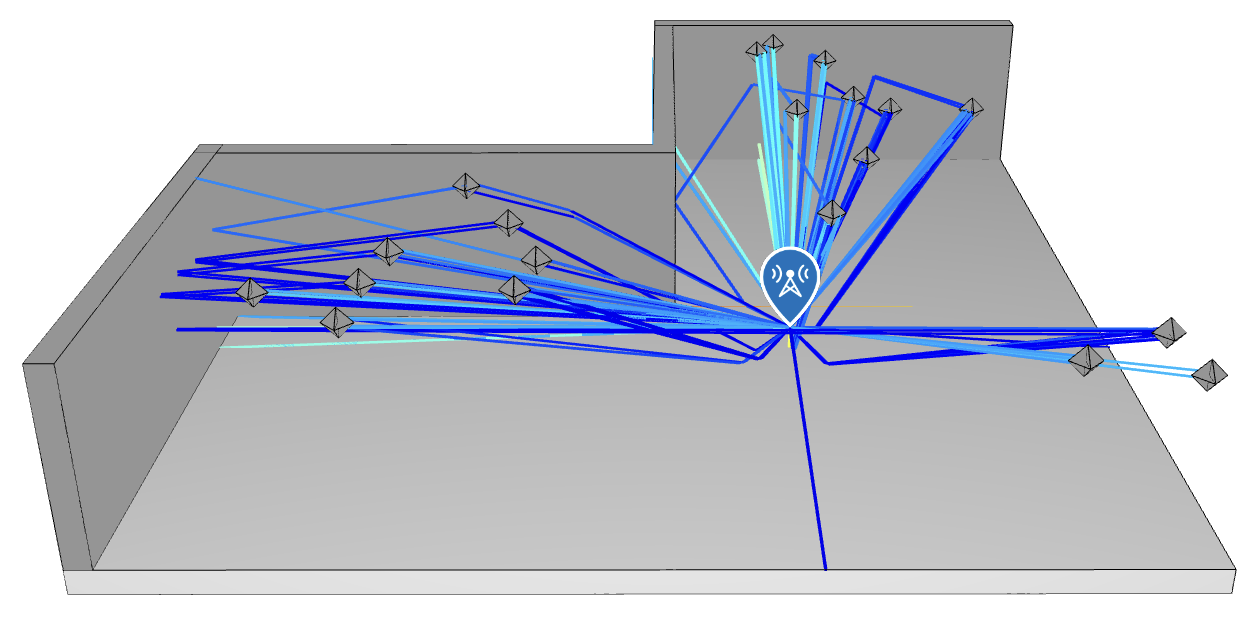
\includegraphics[scale=.28]{figures/thesis_plot.png}
            	\caption{The conceptual view of the millimeter wave indoor localization system}
            \end{figure}
        \item Ray tracing channel simulation
        \item Large and realistic environment
	\end{itemize}
\end{frame}



\begin{frame}[t]{Motivation}
	\begin{itemize}
	    \item Frequency-modulated continuous wave (FMCW) radar
        \vspace{0.5\baselineskip}
            \begin{figure}
            	\centering
            	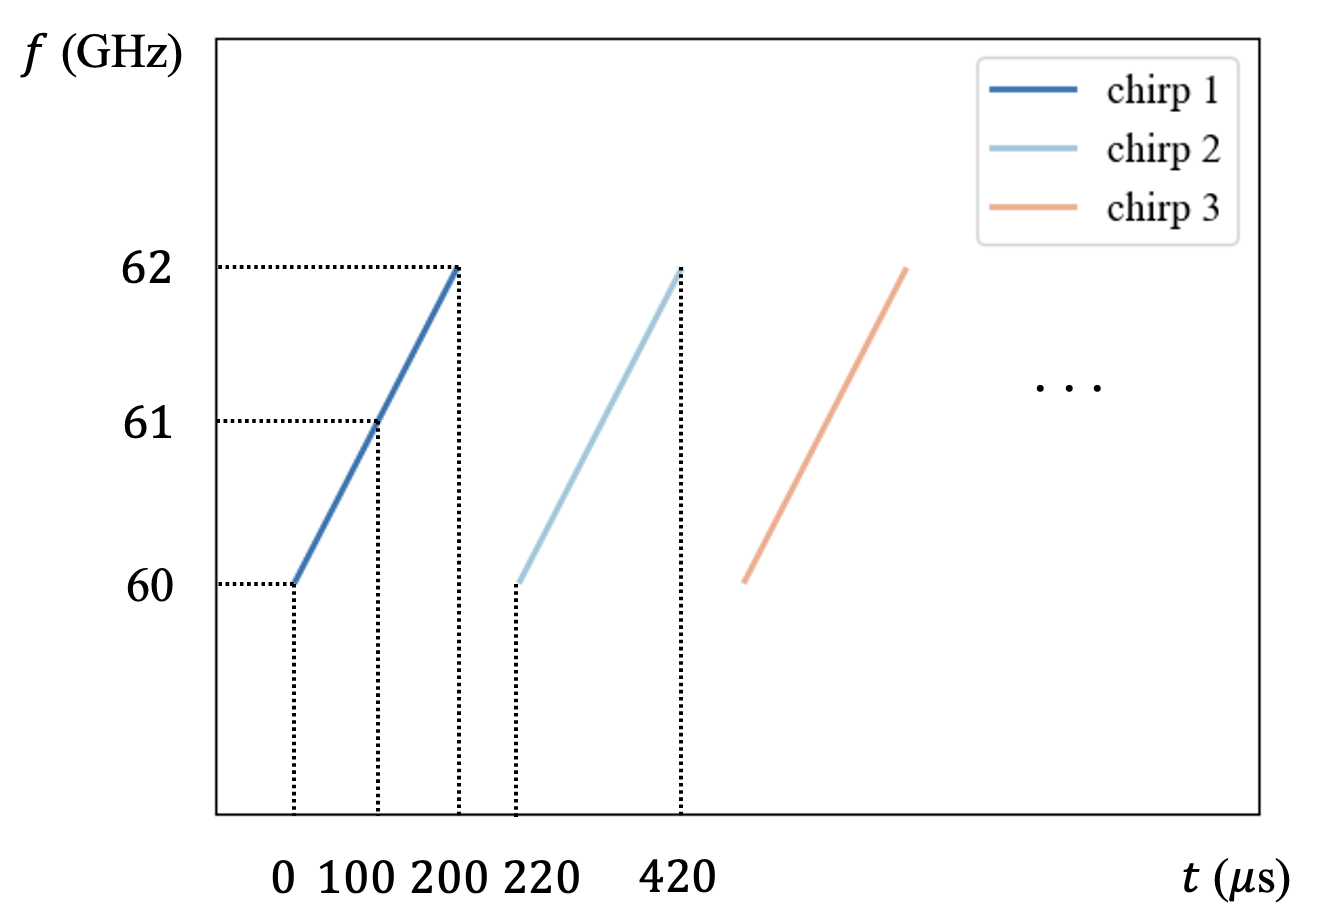
\includegraphics[scale=.3]{figures/FMCW_principle.png}
            	\caption{The principle of the FMCW radar}
            \end{figure}
	\end{itemize}
\end{frame}



% Goal slide
\begin{frame}[t]{Goal}
	\begin{itemize}
	    \item The signal flow
            \begin{figure}
            	\centering
            	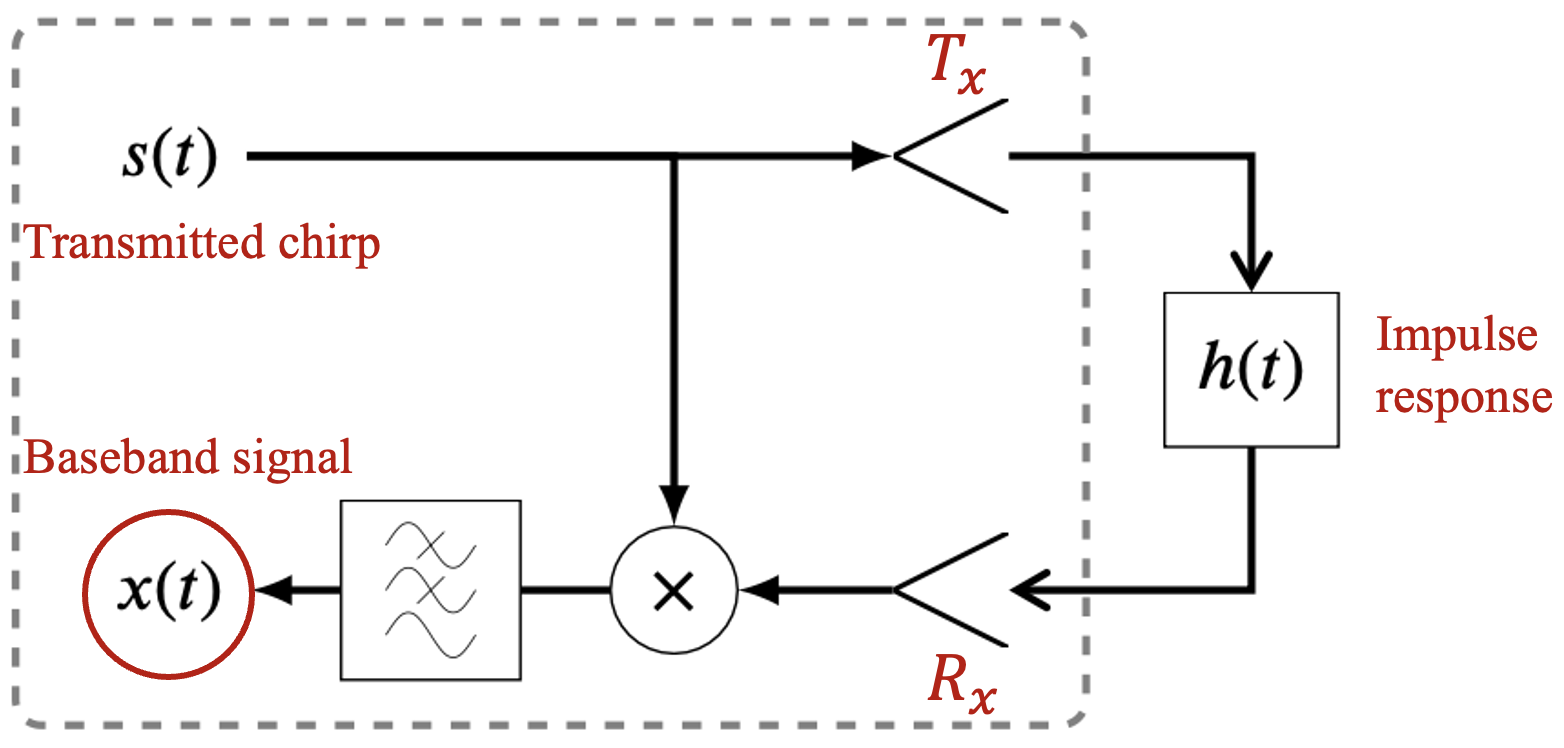
\includegraphics[scale=.3]{figures/signal_flow_pre.png}
            	\caption{The view of the signal flow \cite{hafner_parameter_2021}}
            \end{figure}
        \item Range-Doppler (RD) map and constant false alarm rate (CFAR) detection
	\end{itemize}
\end{frame}

% -----------------------------------------------------------------------------
% This is the table of contents. You can insert a motivation before or after this slide.
\begin{frame}
	\ifthenelse{\equal{\lang}{ngerman}}{
		\frametitle{Inhaltsverzeichnis}
	}{
		\frametitle{Table of Contents}
	}
	\tableofcontents
\end{frame}

% Add an extra slide at the beginning of each section while highlighting the current section
% Use \section* to skip the slide once or comment the following to skip all overview slides.
\AtBeginSection[]
{
	\begin{frame}<beamer>
		\ifthenelse{\equal{\lang}{ngerman}}{
			\frametitle{Inhaltsverzeichnis}
		}{
			\frametitle{Table of Contents}
		}
% 		\frametitle{\contentsname}
		\tableofcontents[currentsection]
	\end{frame}
}

%% =========
\section{Modeling of the channel simulation}
\subsection{Modeling of the room and raytracing}
\setcounter{section}{1}
\setcounter{figure}{0}
% -----------------------------------------------------------------------------
\begin{frame}[t]{Blender}

\begin{itemize}
	\item Modeling of the reflectors
    \vspace{1.0\baselineskip}
    \begin{figure}
        \centering
        \begin{minipage}{0.45\textwidth}
            \centering
            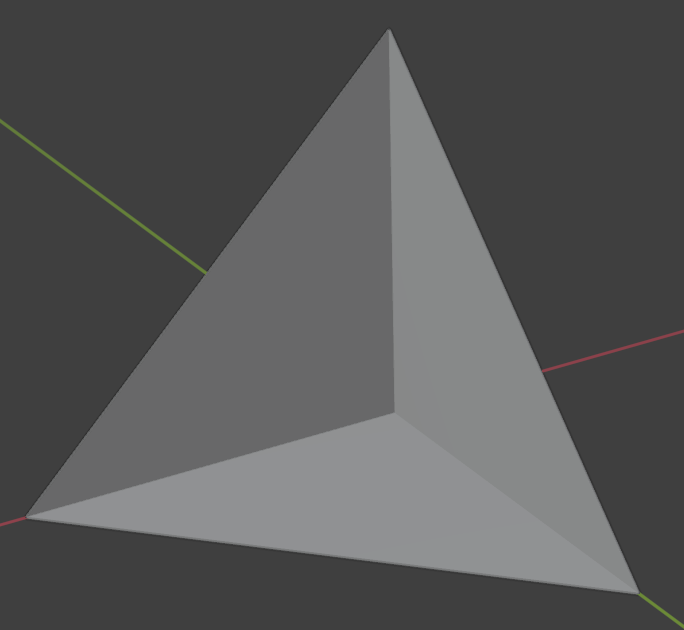
\includegraphics[height=0.5\textheight]{figures/tri_reflector.png}
            \caption{Trihedral corner reflector}
        \end{minipage}
        \begin{minipage}{0.45\textwidth}
            \centering
            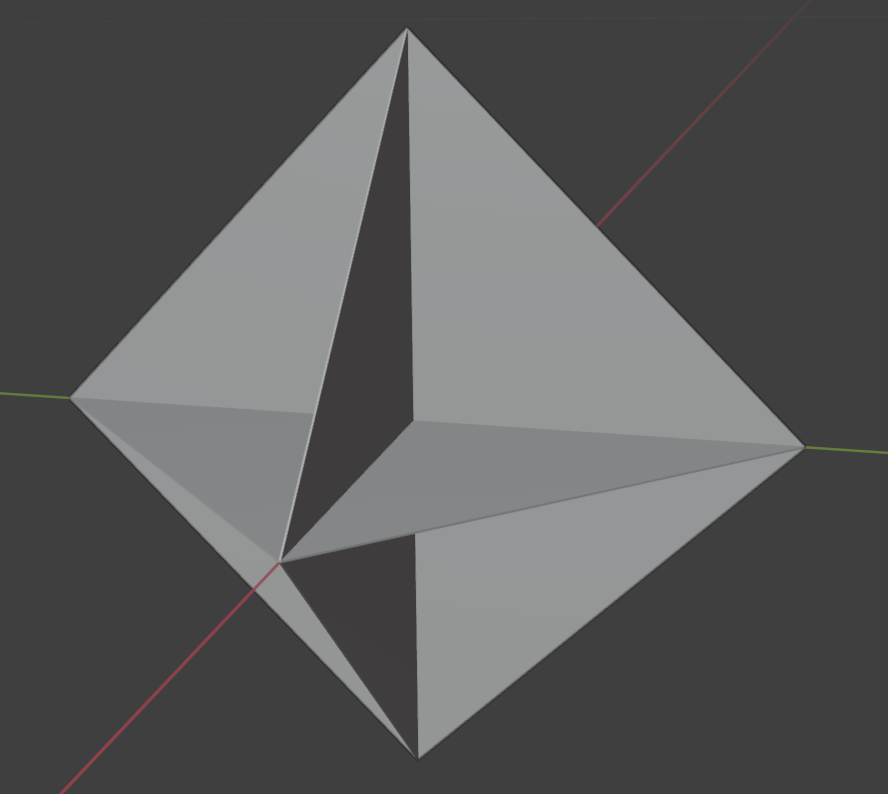
\includegraphics[height=0.5\textheight]{figures/octa_reflector.png}
            \caption{Octahedral reflector}
        \end{minipage}
    \end{figure}
\end{itemize}
\end{frame}


\begin{frame}[t]{Blender}

\begin{itemize}
	\item Modeling of the room model
    \vspace{1.0\baselineskip}
    \begin{figure}
        \centering
        \begin{minipage}{0.45\textwidth}
            \centering
            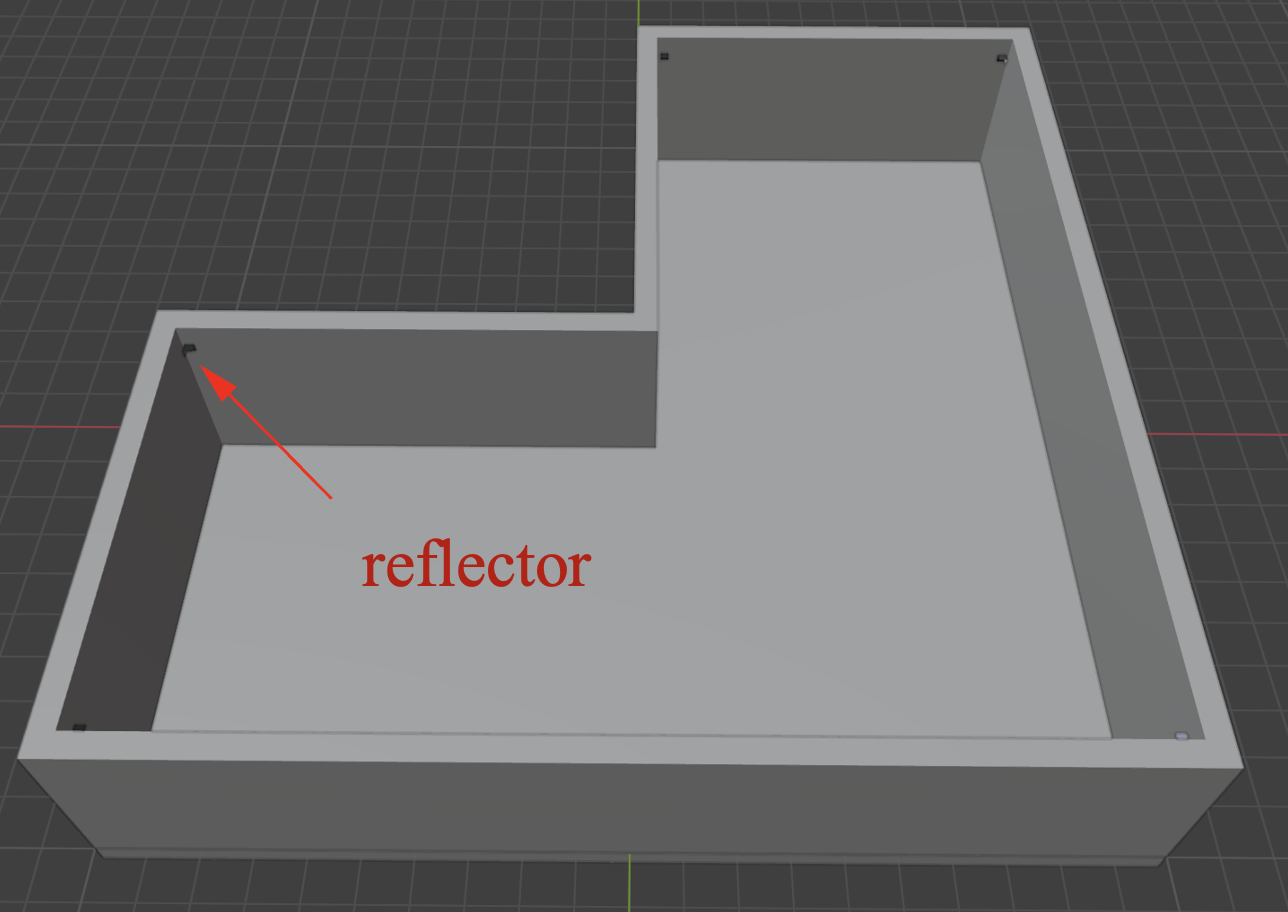
\includegraphics[height=0.7\textwidth]{figures/empty_room_without_ceiling.png}
            \caption{Room model with reflectors}
        \end{minipage}
        \begin{minipage}{0.45\textwidth}
            \centering
            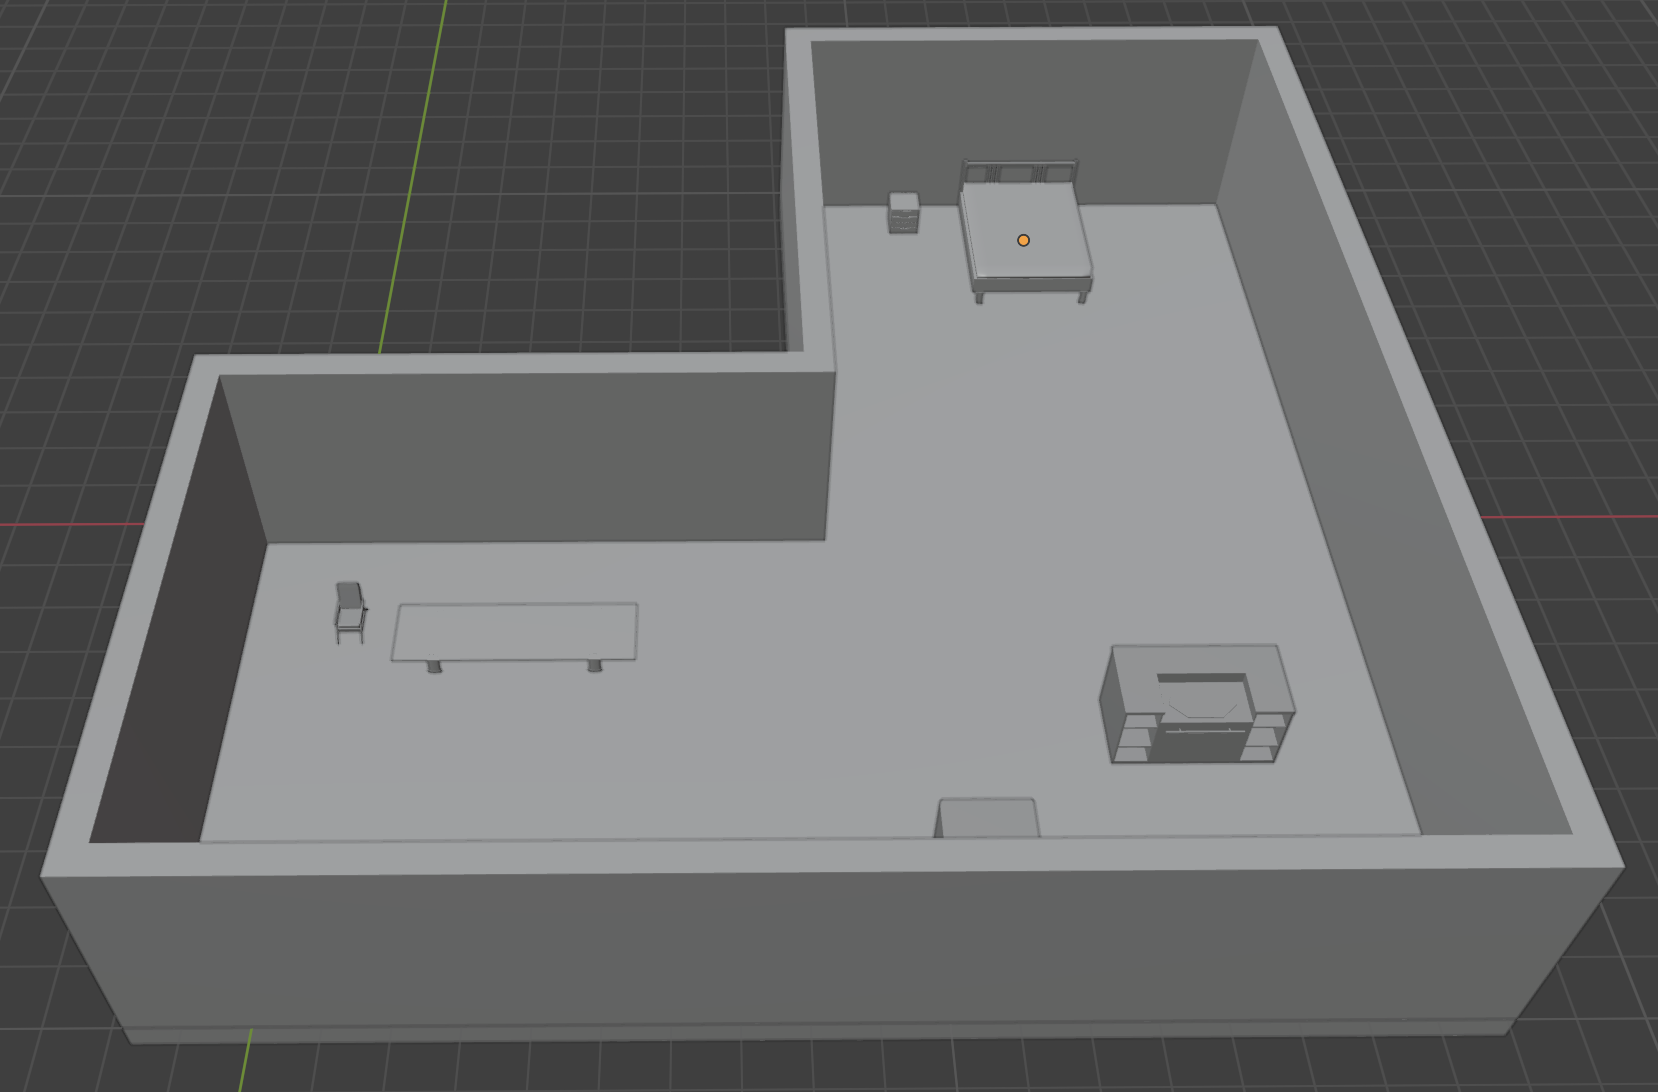
\includegraphics[height=0.7\textwidth]{figures/furniture_simple.png}
            \caption{Room model with furniture \cite{blender_furniture}}
        \end{minipage}
    
    \end{figure}
\end{itemize}
\end{frame}



\begin{frame}[t]{Raytracer}
	\begin{itemize}
        \item Setup of the raytracing (MaxNumreflections, MaxAbsolutePathLoss, Method, etc.)
	    \item The shooting and bouncing ray (SBR) method
        \vspace{0.5\baselineskip}
            \begin{figure}
            	\centering
            	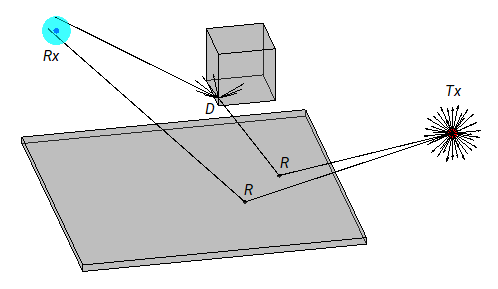
\includegraphics[scale=.5]{figures/ray_tracing_sbr_method.png}
            	\caption{The view of the SBR method \cite{ray_tracer_inputs}}
            \end{figure}
	\end{itemize}
\end{frame}





\begin{frame}[t]{Raytracing}
	\begin{itemize}
	    \item The view of raytracing in the empty room model and room model with furniture
        \vspace{0.5\baselineskip}
            \begin{figure}
                \centering
                \begin{minipage}{0.45\textwidth}
                    \centering
                    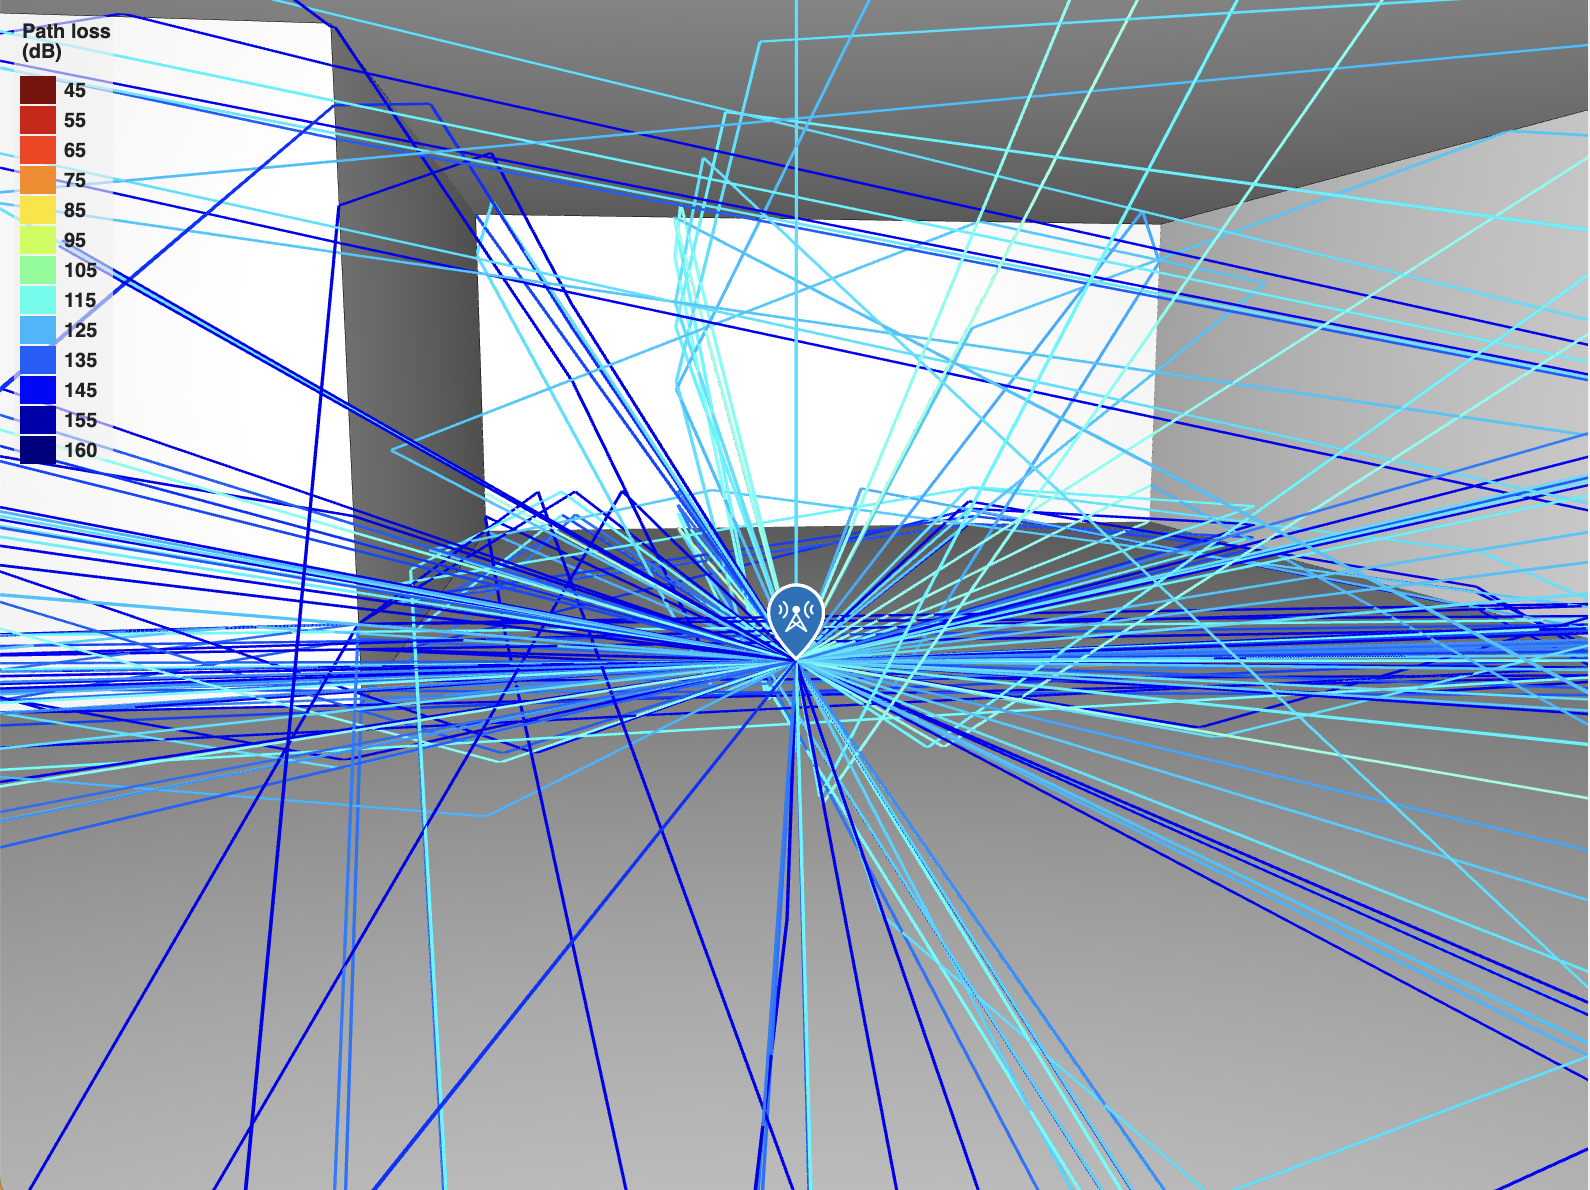
\includegraphics[height=0.7\textwidth]{figures/empty_room_simulation_right.png}
                    \caption{In empty room model}
                \end{minipage}
                \begin{minipage}{0.45\textwidth}
                    \centering
                    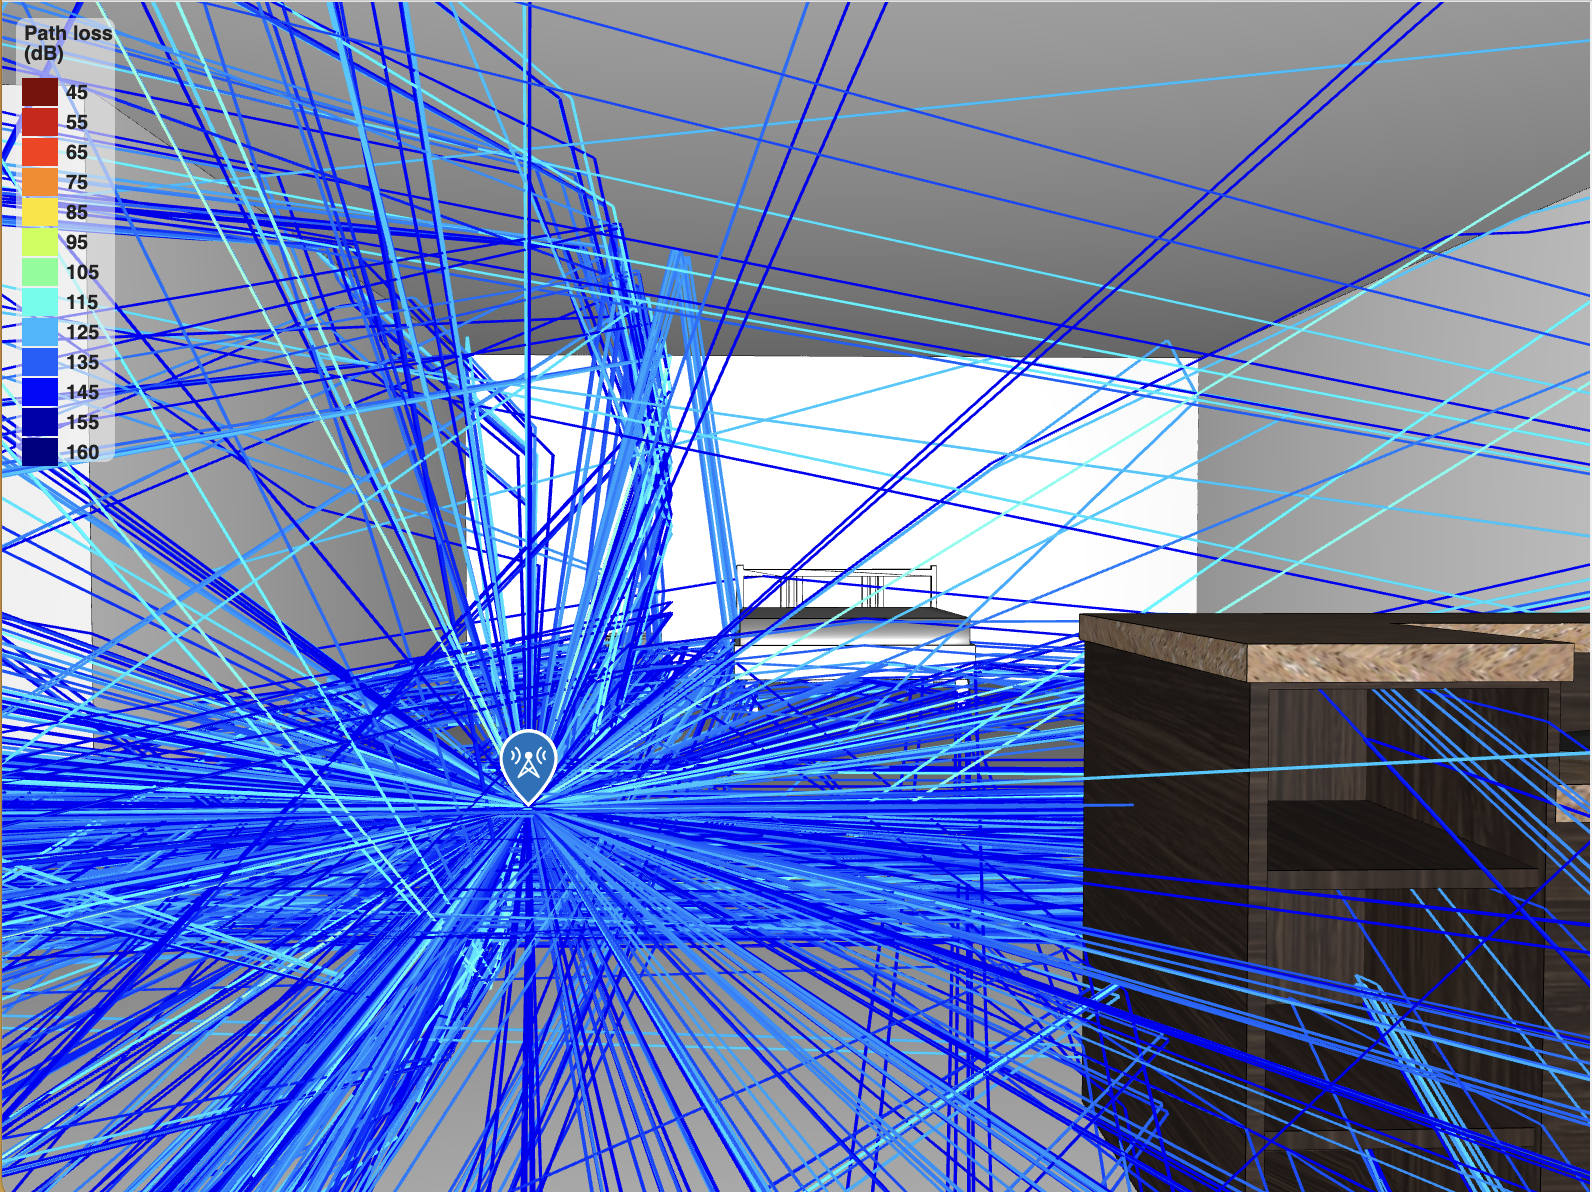
\includegraphics[height=0.7\textwidth]{figures/furniture_simulation_right.png}
                    \caption{In room with furniture}
                \end{minipage}
            \end{figure}
	\end{itemize}
\end{frame}



\begin{frame}[t]{Raytracer}
	\begin{itemize}
	    \item The view of raytracing in the room model with reflectors and inside the reflector
        \vspace{0.5\baselineskip}
            \begin{figure}
                \centering
                \begin{minipage}{0.45\textwidth}
                    \centering
                    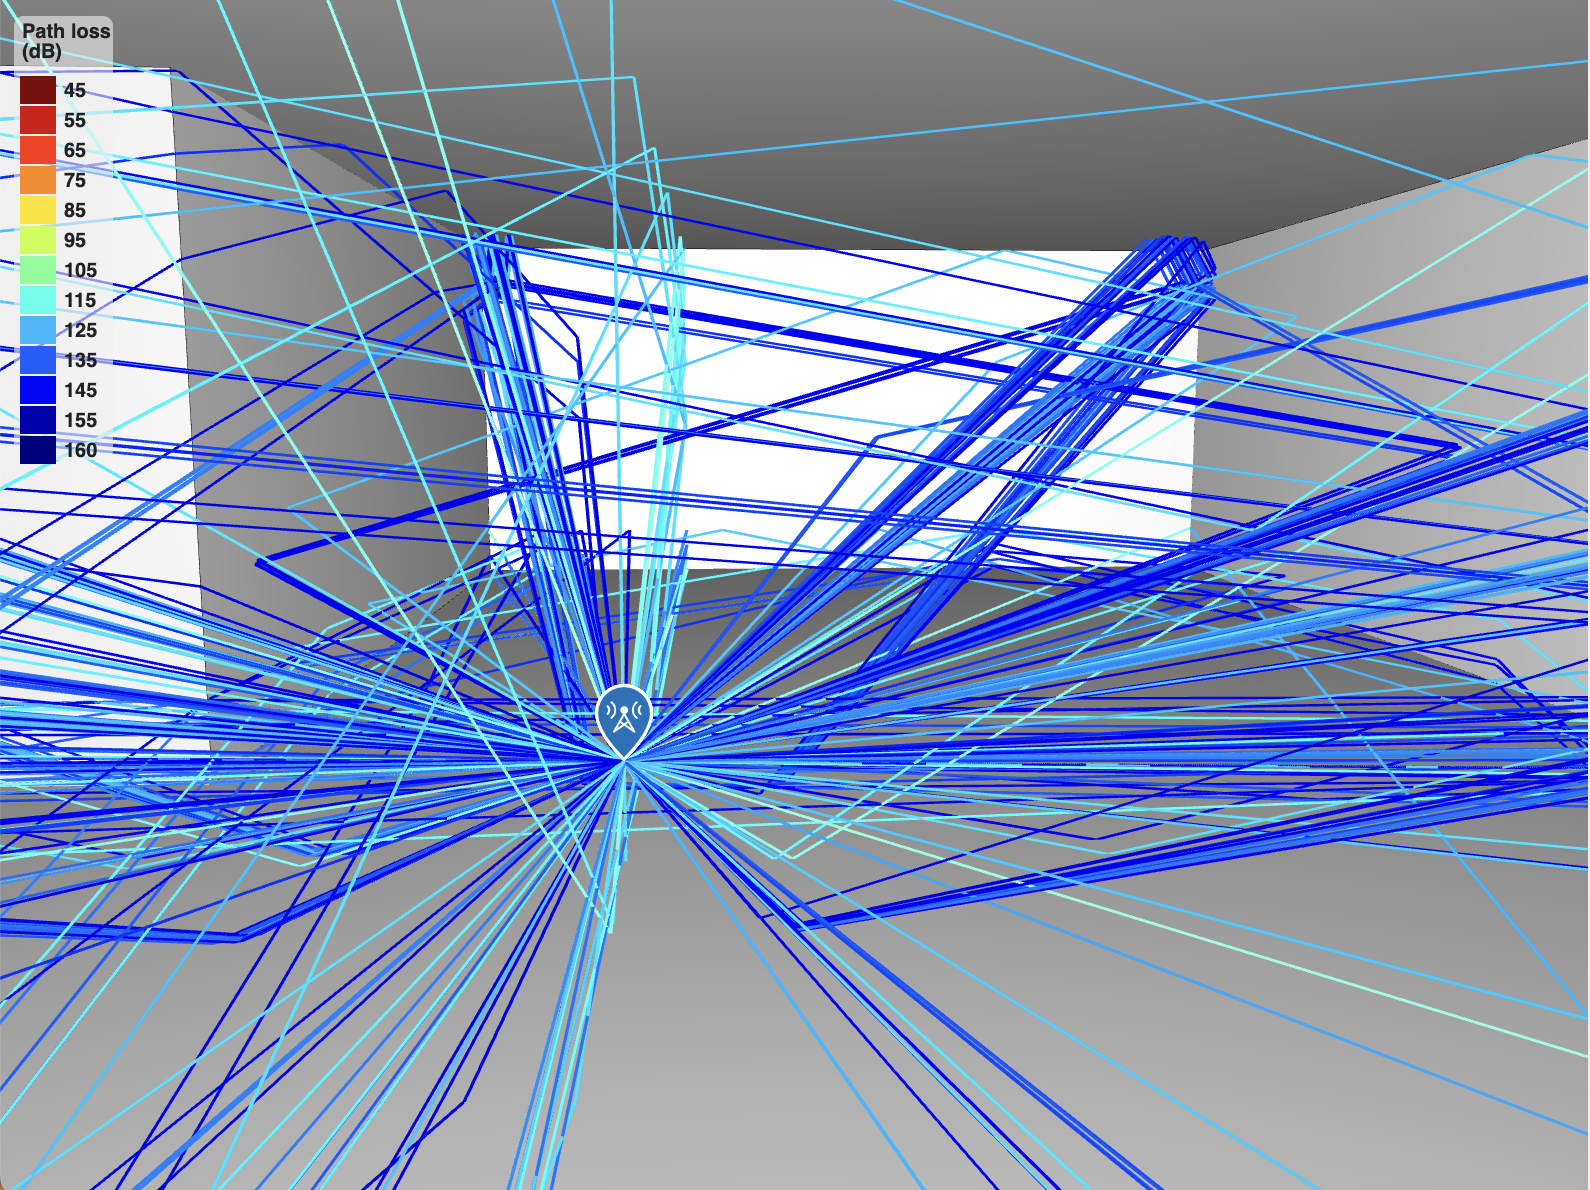
\includegraphics[height=0.7\textwidth]{figures/reflector_simulation_right.png}
                    \caption{In room with reflectors}
                \end{minipage}
                \begin{minipage}{0.45\textwidth}
                    \centering
                    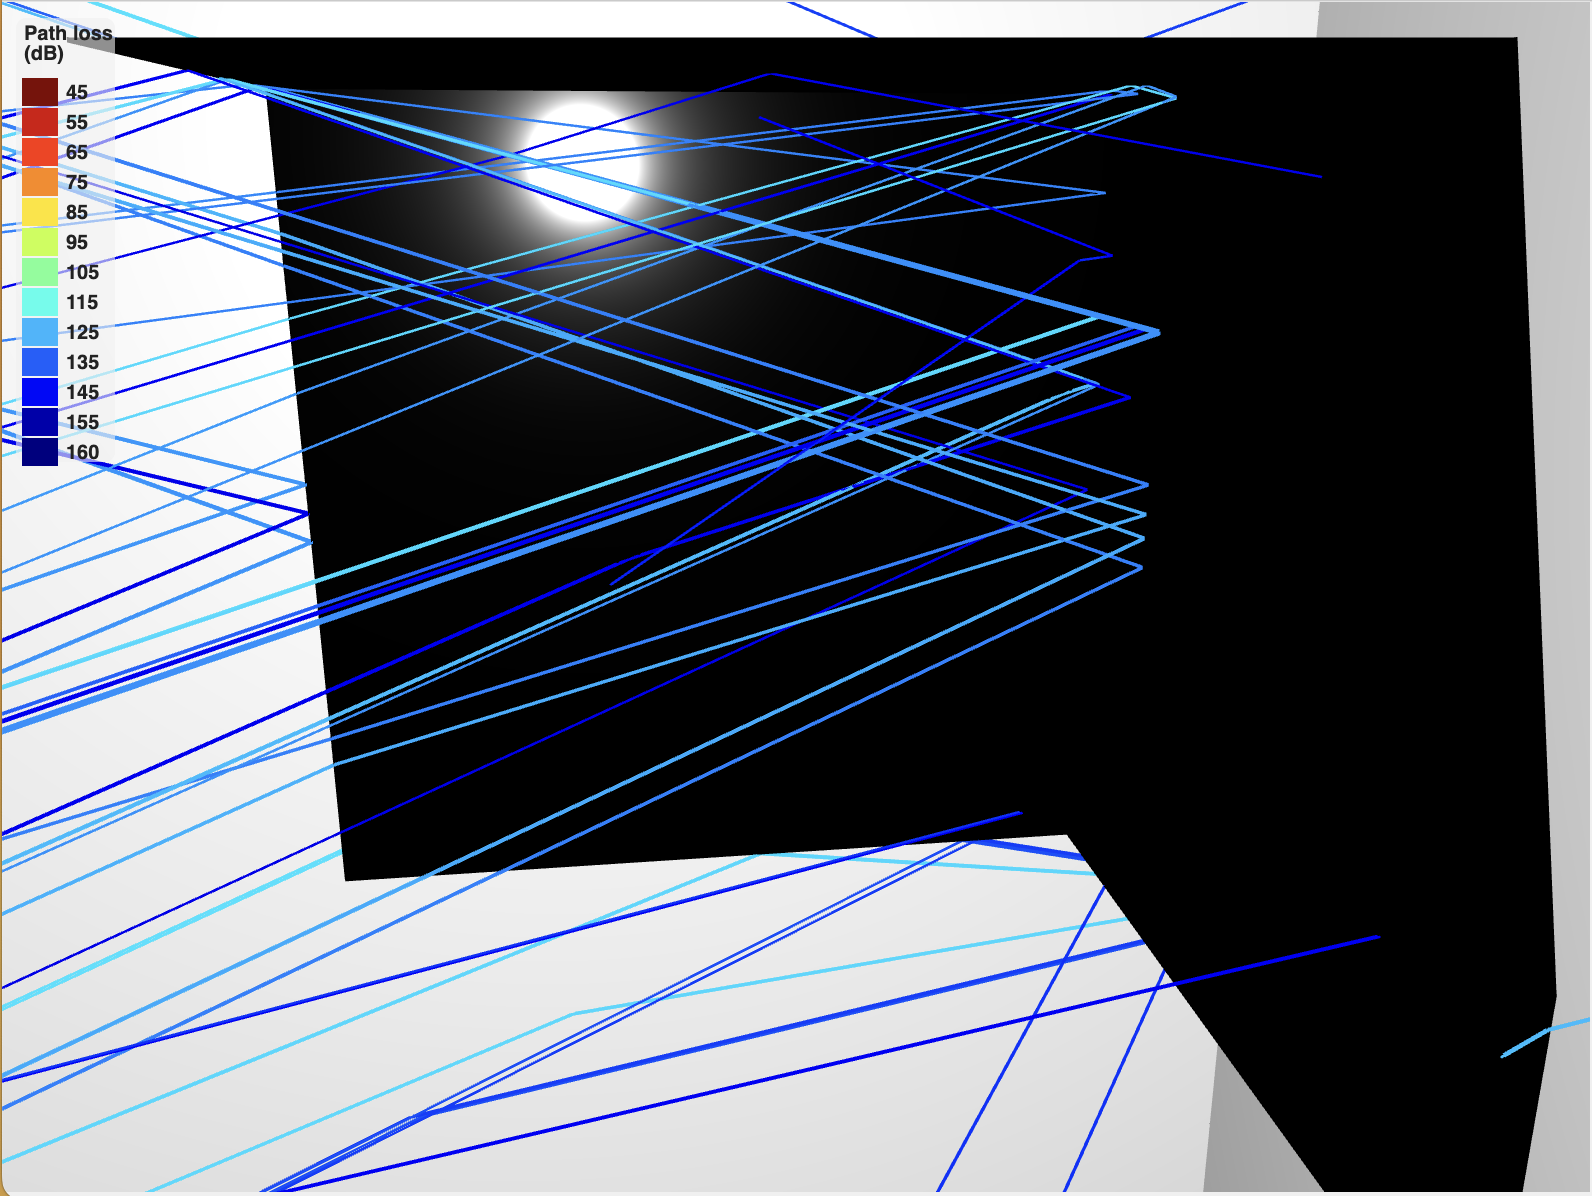
\includegraphics[height=0.7\textwidth]{figures/reflections_inside_reflector.png}
                    \caption{The view inside the reflector}
                \end{minipage}
            \end{figure}
	\end{itemize}
\end{frame}


\subsection{LOS rays between the reflectors and radar}
% -----------------------------------------------------------------------------
\begin{frame}[t]{Line-of-sight (LOS) rays}
    \begin{itemize}
	    \item Setting the receivers at the positions of reflectors to obtain LOS rays
        \vspace{0.5\baselineskip}
            \begin{figure}
                \centering
                \begin{minipage}{0.45\textwidth}
                    \centering
                    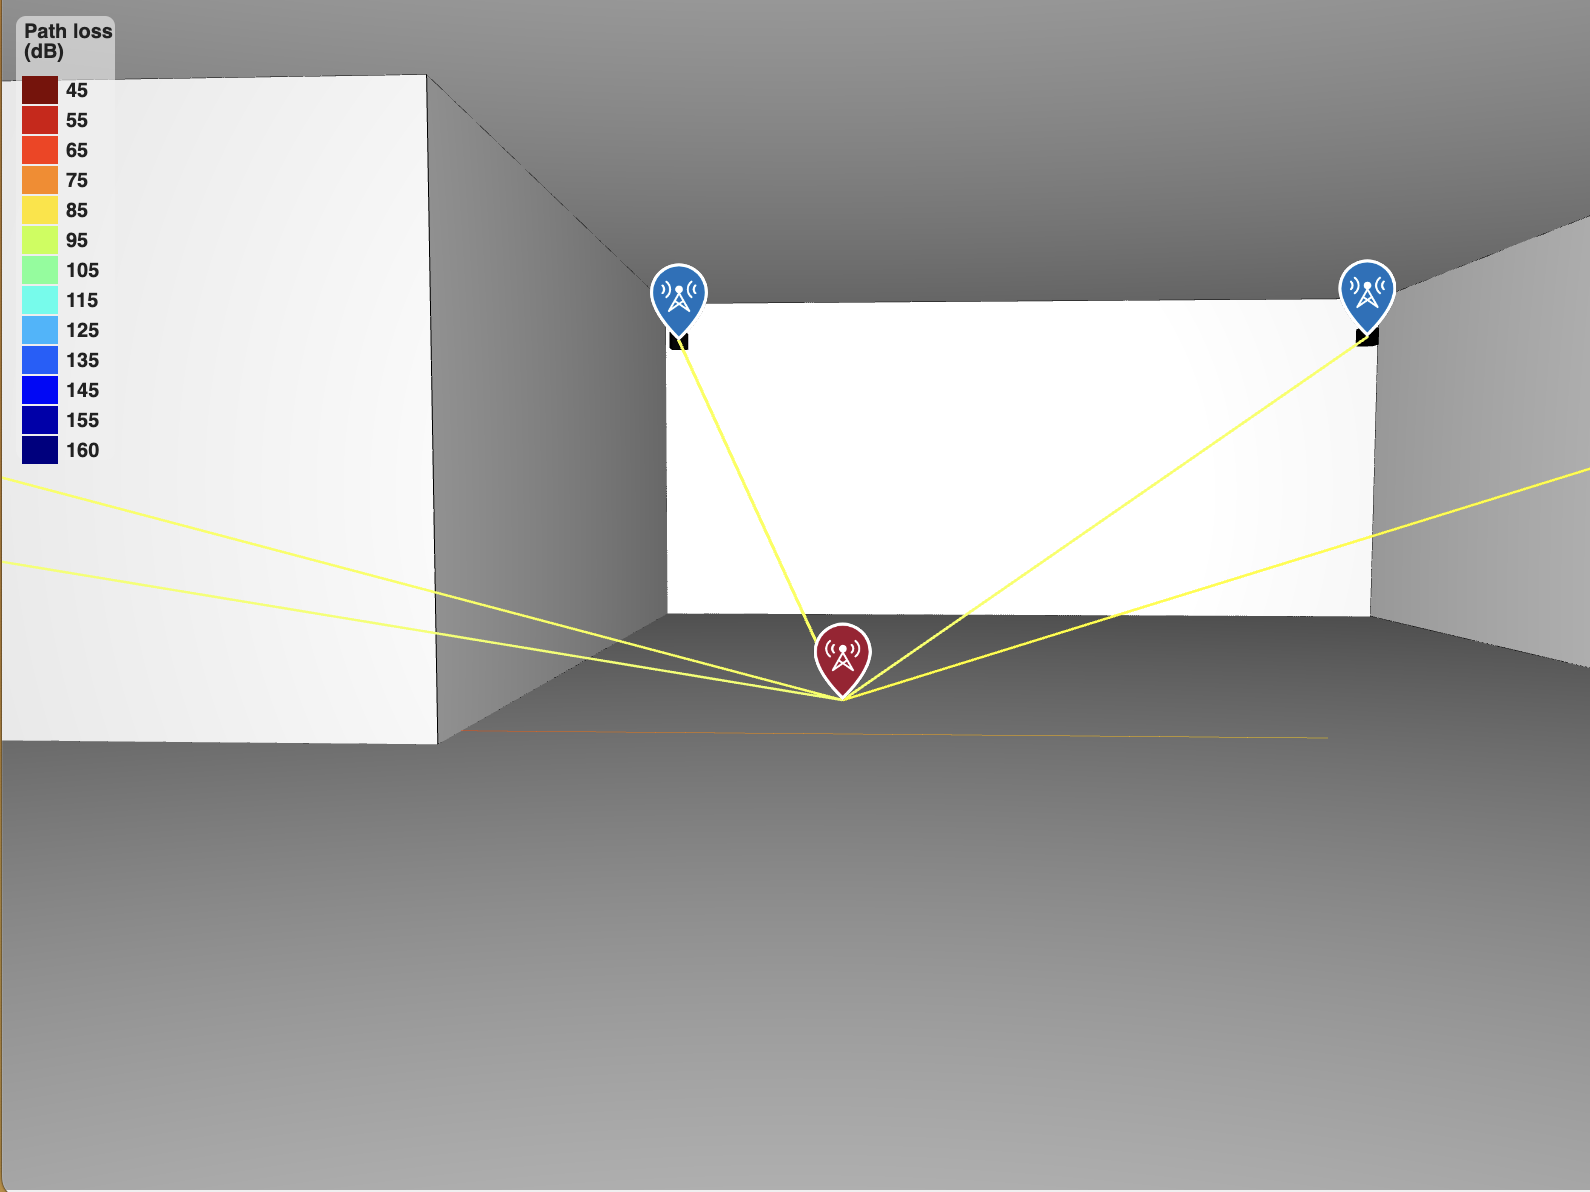
\includegraphics[height=0.7\textwidth]{figures/LOS_5_reflectors.png}
                    \caption{LOS rays from five trihedral corner reflectors}
                \end{minipage}
                \begin{minipage}{0.45\textwidth}
                    \centering
                    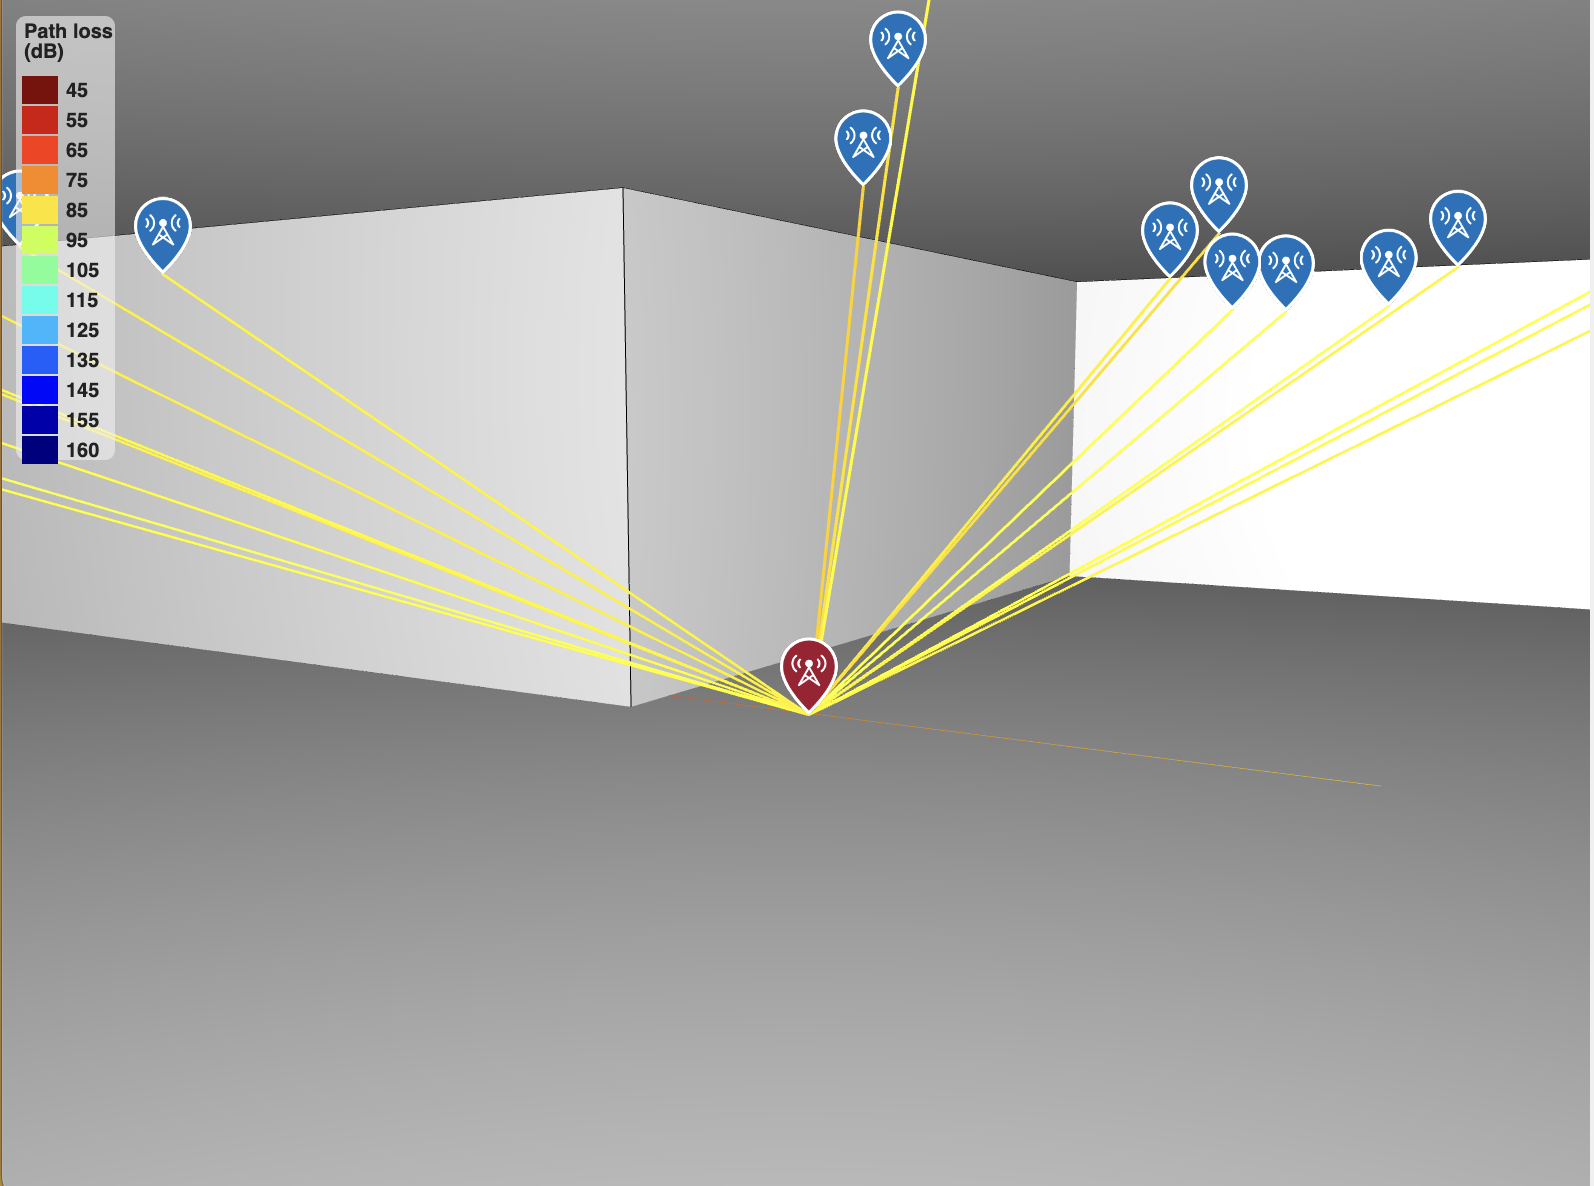
\includegraphics[height=0.7\textwidth]{figures/LOS_more_reflectors.png}
                    \caption{LOS rays from multiple octahedral reflectors}
                \end{minipage}
            \end{figure}
	\end{itemize}
\end{frame}



\begin{frame}[t]{Path loss (PL)}
    \begin{equation}
        \centering
        PL = 10\cdot\log_{10}\left(\frac{G_{T}G_{R}\lambda^{2}\cdot\sigma}{(4\pi)^{3} r^{4}}\right) \cite{richards_principles_2010},
        \label{path loss formula}
    \end{equation}
    where
    \begin{itemize}
        \item $G_T$ and $G_R$ are the gain values of transmitter and receiver respectively.
        \item $\lambda$ is the wavelength of the ray.
        \item $\sigma$ is the radar cross section.
        \item $r$ represents the propagation distance of LOS rays.
    \end{itemize}
\end{frame}




\subsection{Signal processing}
% -----------------------------------------------------------------------------
\begin{frame}[t]{The signal model}
    \begin{equation}
        \centering
        x(n_s, n_p) = \sum_{m} A_m \exp \left( 2\pi j \left(\frac{2 B r_{m}}{T_c c} T_s n_s + \frac{2 f v_{m}}{c} T_p n_p \right) \right) + n(n_s, n_p)\,\mathrm{\cite{ouza_simple_2017}},
    \end{equation}
    where
    \begin{itemize}
        \item $x(n_s, n_p)$ is an element of a 2D matrix $\mathbf{X}$, i.e. baseband signal,
        \item $n_s$ = 1...256 is the fast time samples,
        \item $n_p$=1...32 is the slow time samples,
        \item $m$ represents each ray in the channel simulation,
        \item $A_m = \sqrt{P_T \cdot 10^{-PL_m / 10} \cdot R}$,
        \item the first term for the delay and the second term for the Doppler effect,
        \item $n(n_s, n_p)$ is the Gaussian noise $n \sim \mathcal{CN}(0, V_{noise})$.
    \end{itemize}
\end{frame}


\begin{frame}[t]{Range-Doppler map}
    \begin{itemize}
        \item The view of 2D fast Fourier transform (FFT) and range-Doppler map
         \vspace{0.5\baselineskip}
            \begin{figure}
                \centering
                \begin{minipage}{0.45\textwidth}
                    \centering
                    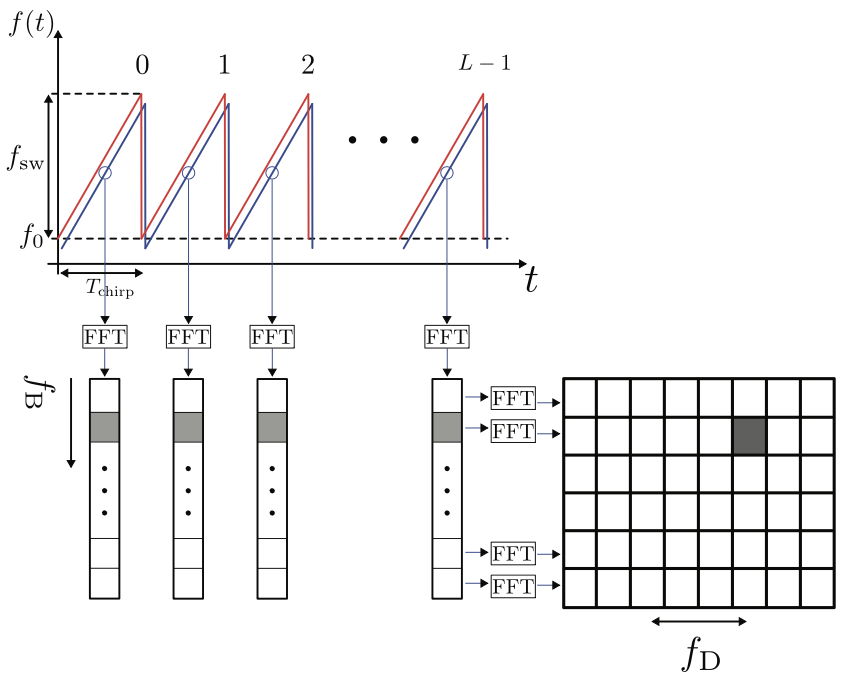
\includegraphics[height=0.8\textwidth]{figures/2D_FFT.png}
                    \caption{The view of 2D FFT \cite{kronauge_new_2014}}
                \end{minipage}
                \begin{minipage}{0.45\textwidth}
                    \centering
                    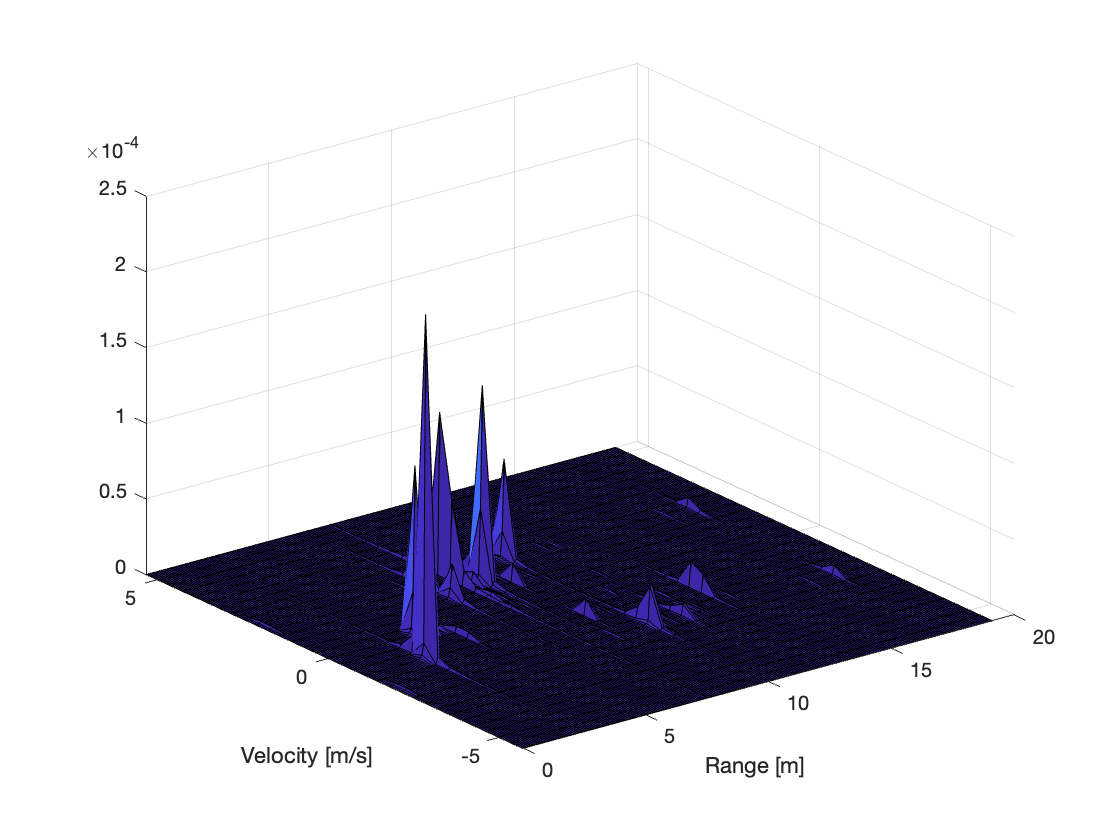
\includegraphics[height=0.8\textwidth]{figures/2r_furniture.png}
                    \caption{Range-Doppler map}
                \end{minipage}
            \end{figure}
    \end{itemize}
\end{frame}



\begin{frame}[t]{Constant false alarm rate (CFAR) detection}
	\begin{itemize}
        \item The CFAR plots for the empty room model and room model with reflectors
         \vspace{0.5\baselineskip}
            \begin{figure}
                \centering
                \begin{minipage}{0.45\textwidth}
                    \centering
                    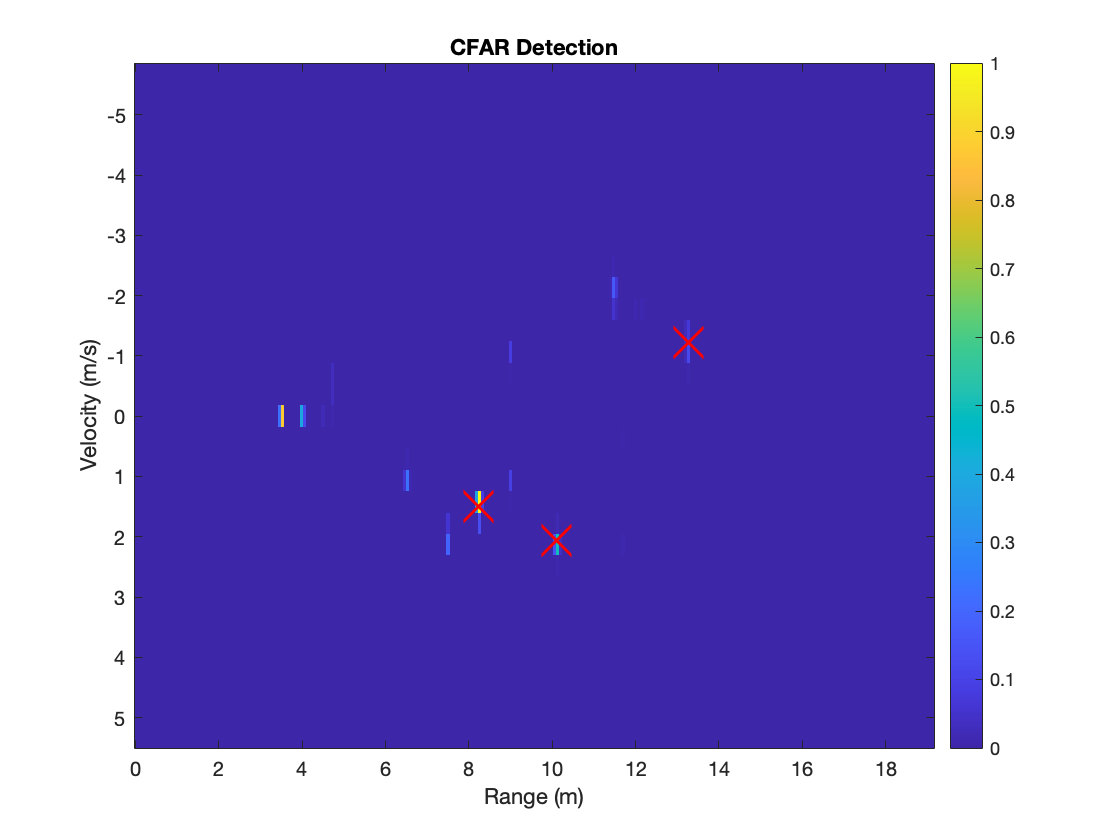
\includegraphics[height=0.8\textwidth]{figures/2c_empty_pre.png}
                    \caption{In the empty room}
                \end{minipage}
                \begin{minipage}{0.45\textwidth}
                    \centering
                    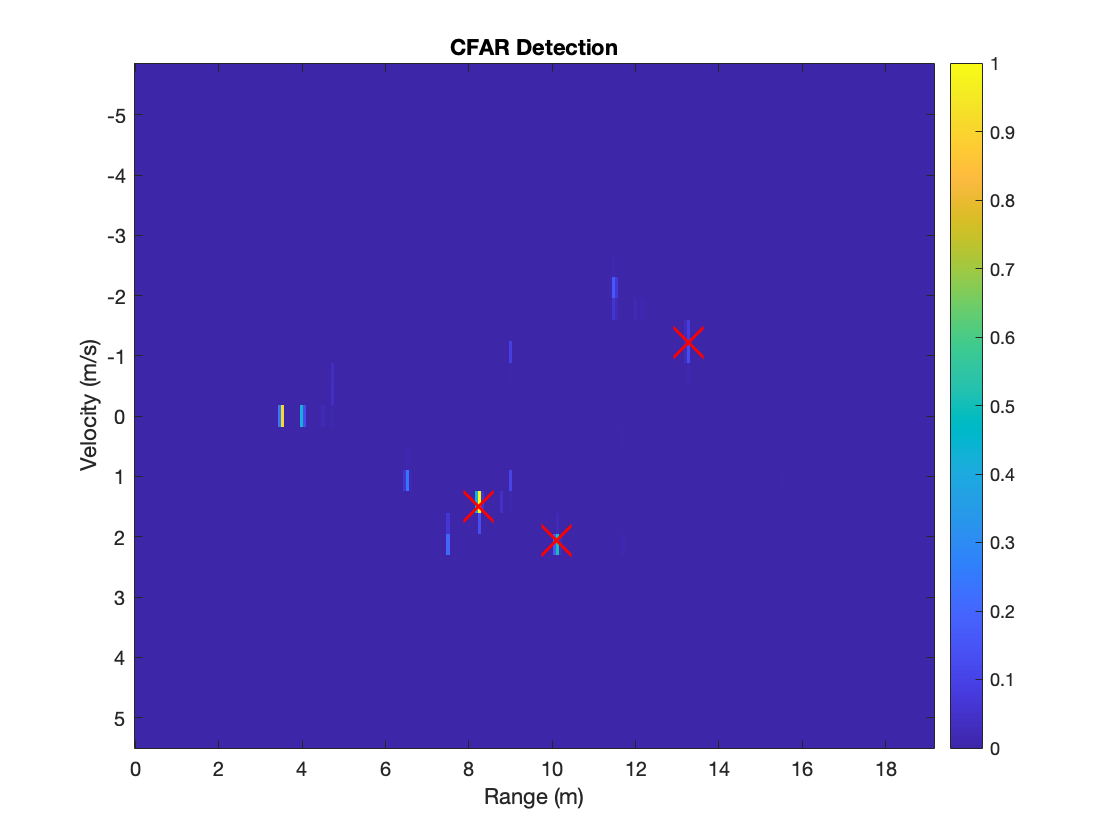
\includegraphics[height=0.8\textwidth]{figures/2c_reflectors_pre.png}
                    \caption{In the room with reflectors}
                \end{minipage}
            \end{figure}
    \end{itemize}
\end{frame}




\begin{frame}[t]{Constant false alarm rate (CFAR) detection}
	\begin{itemize}
        \item The CFAR plots for the room model with reflectors and with furniture
         \vspace{0.5\baselineskip}
            \begin{figure}
                \centering
                \begin{minipage}{0.45\textwidth}
                    \centering
                    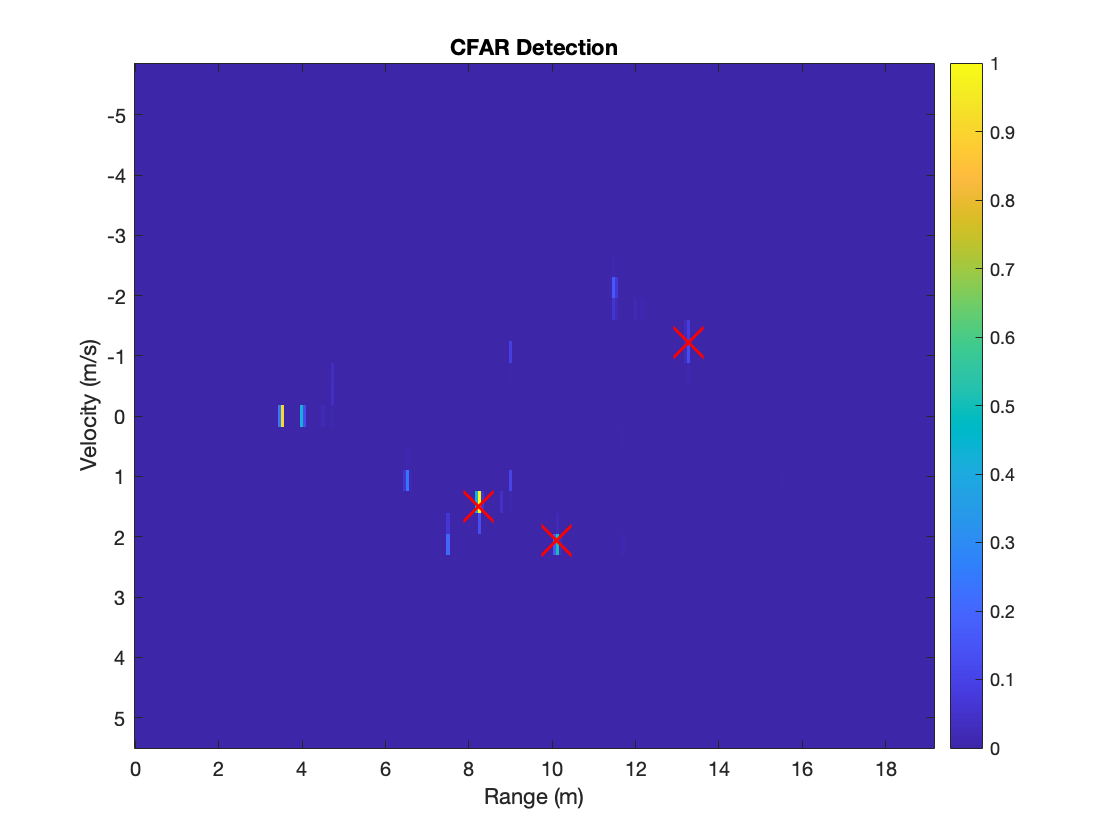
\includegraphics[height=0.8\textwidth]{figures/2c_reflectors_pre.png}
                    \caption{In the room with reflectors}
                \end{minipage}
                \begin{minipage}{0.45\textwidth}
                    \centering
                    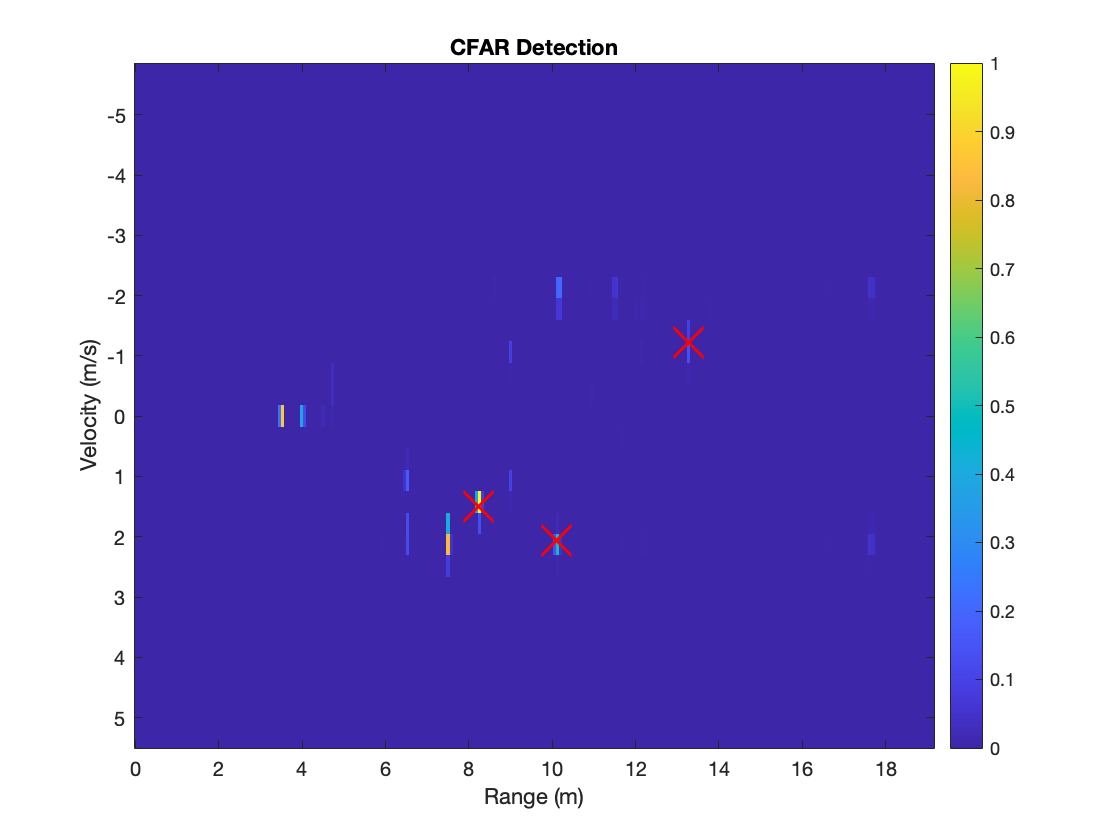
\includegraphics[height=0.8\textwidth]{figures/2c_furniture_pre.png}
                    \caption{In the room with furniture}
                \end{minipage}
            \end{figure}
    \end{itemize}
\end{frame}




\section{Antenna radiation pattern}
\subsection{Antenna designer}
\setcounter{section}{2}
\setcounter{figure}{0}
% -----------------------------------------------------------------------------

\begin{frame}[t]{Antenna designer}
	\begin{itemize}
	    \item "Optimization" function to obtain maximum gain value
        \vspace{1.0\baselineskip}
            \begin{figure}
            	\centering
            	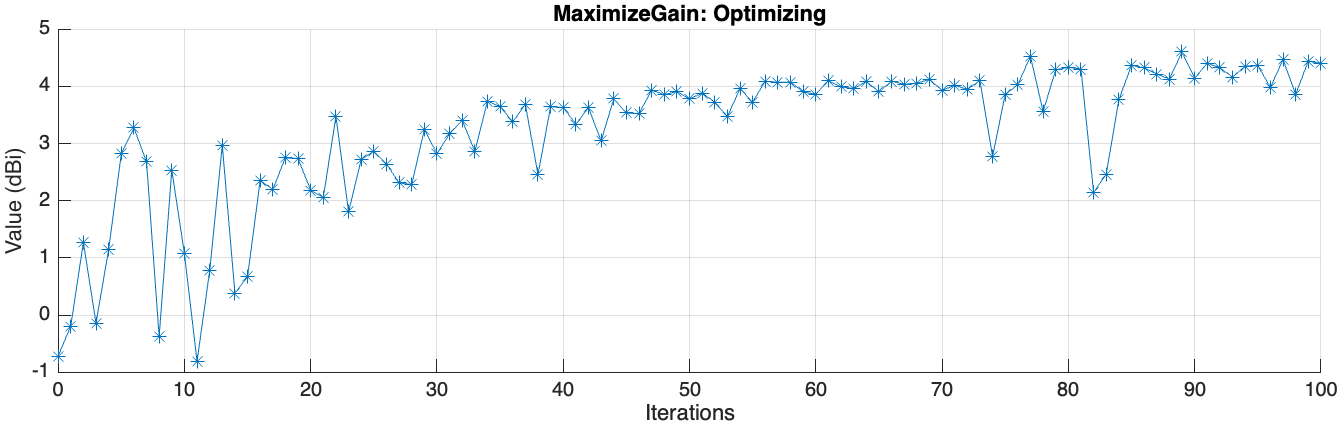
\includegraphics[scale=.5]{figures/max_gain.png}
            	\caption{The view of the maximum gain}
            \end{figure}
	\end{itemize}
\end{frame}




\begin{frame}[t]{Antenna designer}
	\begin{itemize}
	    \item The gain as $az=0^{\circ}$ between the first version and after tuning
        \vspace{1.0\baselineskip}
            \begin{figure}
                \centering
                \begin{minipage}{0.45\textwidth}
                    \centering
                    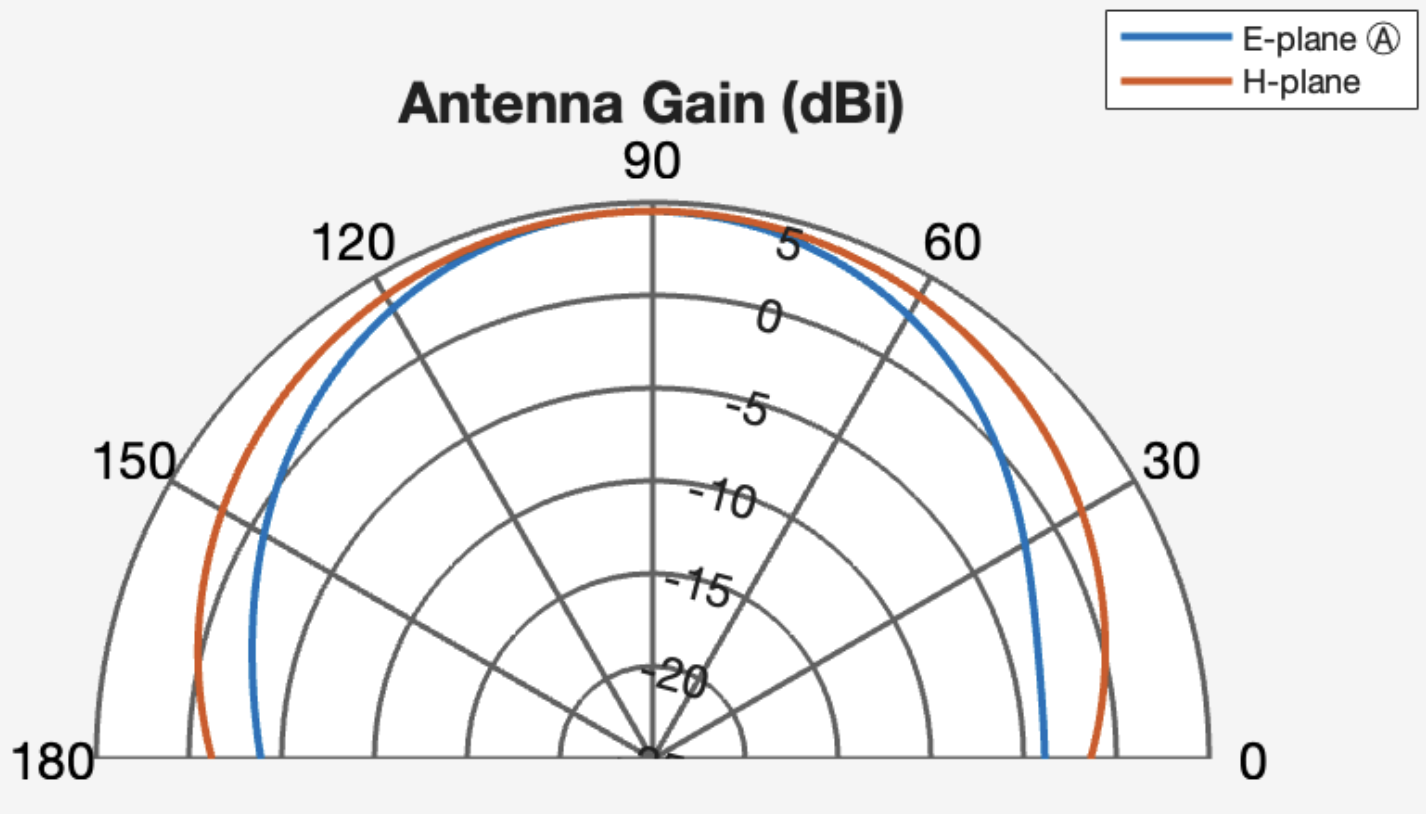
\includegraphics[height=0.55\textwidth]{figures/antenna_gain_optimization.png}
                    \caption{The gain of the first version}
                \end{minipage}
                \begin{minipage}{0.45\textwidth}
                    \centering
                    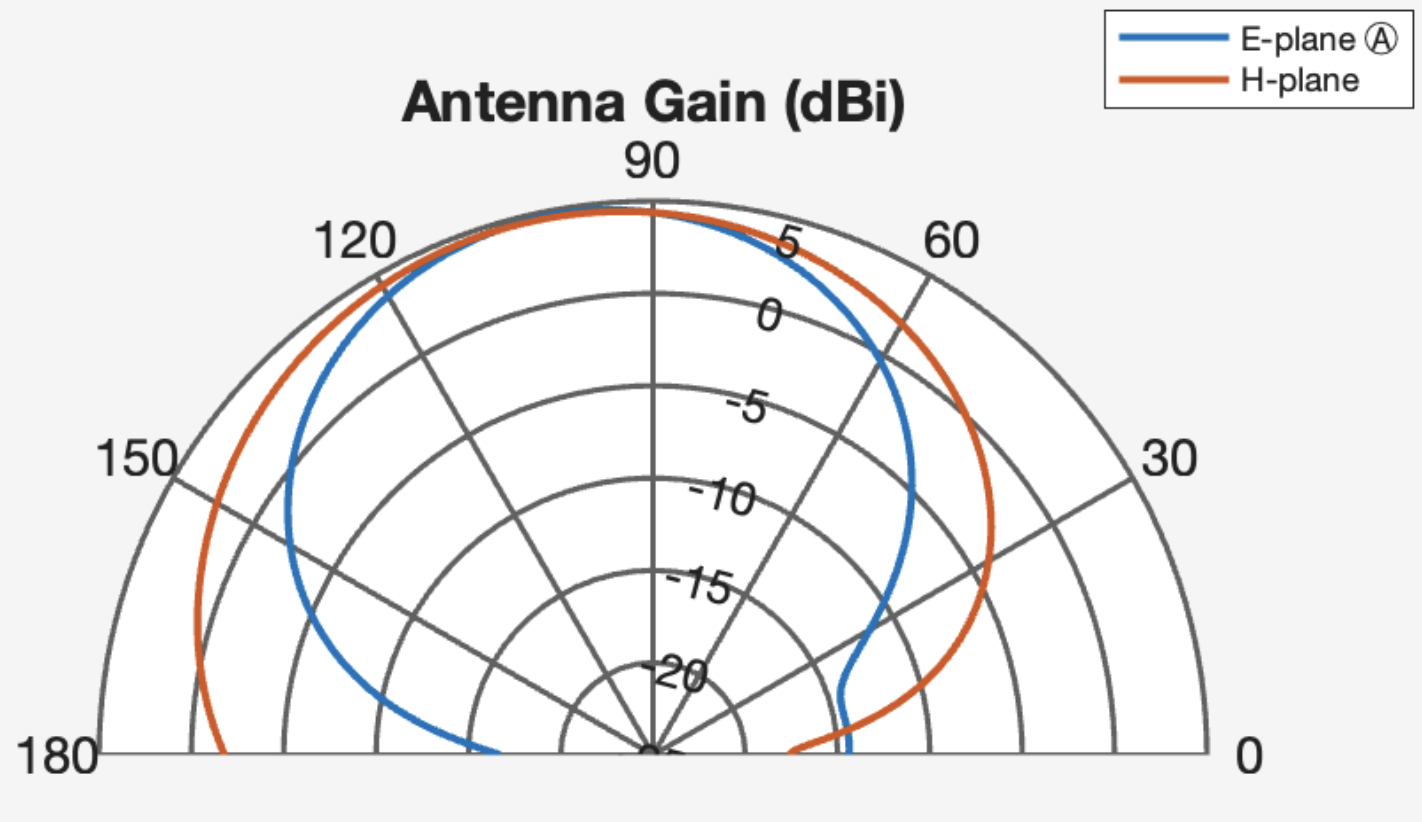
\includegraphics[height=0.55\textwidth]{figures/antenna_gain_latest.png}
                    \caption{The gain after tuning}
                \end{minipage}
            \end{figure}
	\end{itemize}
\end{frame}




\begin{frame}[t]{Antenna designer}
	\begin{itemize}
	    \item The view and radiation pattern of the final antenna
        \vspace{1.5\baselineskip}
            \begin{figure}
                \centering
                \begin{minipage}{0.45\textwidth}
                    \centering
                    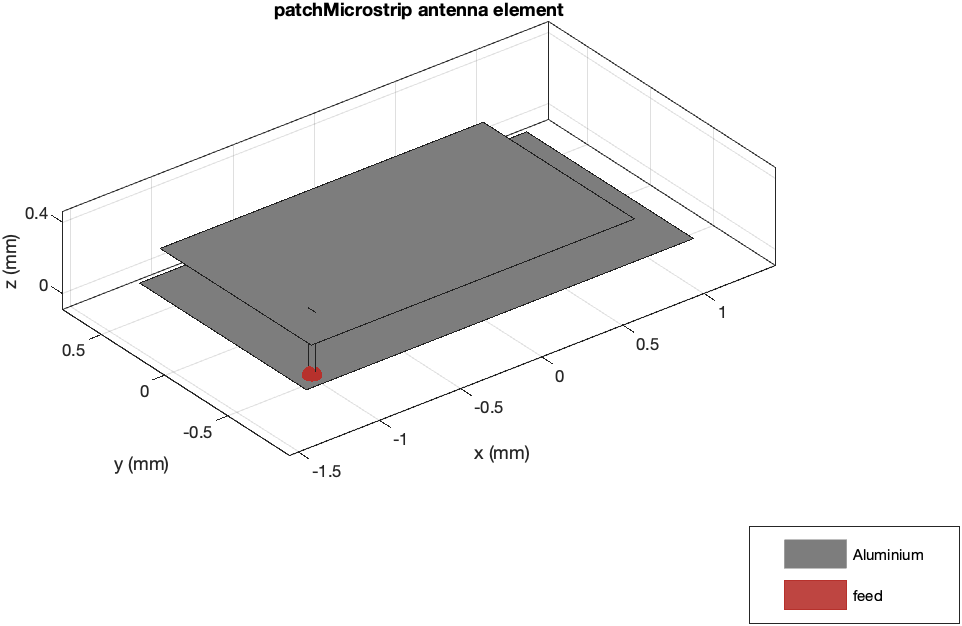
\includegraphics[height=0.6\textwidth]{figures/antenna_plot_latest.png}
                    \caption{View of the final antenna}
                \end{minipage}
                \begin{minipage}{0.45\textwidth}
                    \centering
                    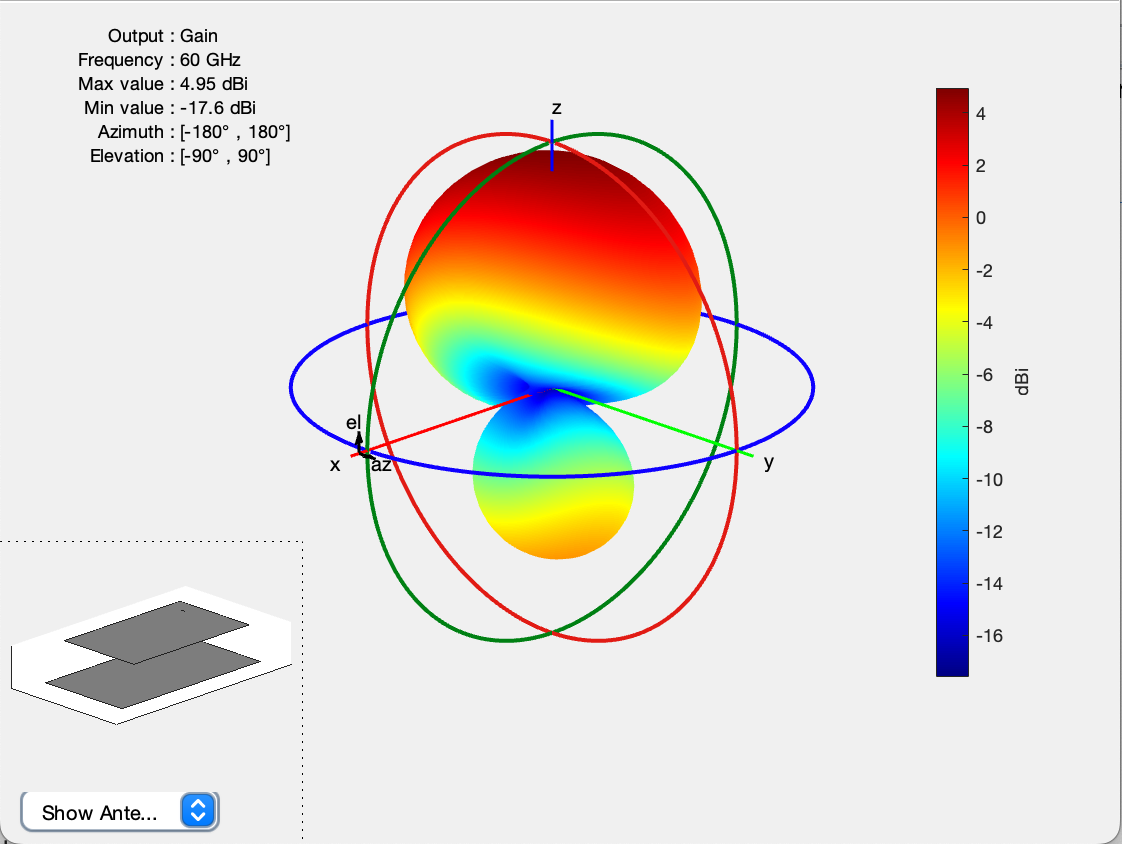
\includegraphics[height=0.6\textwidth]{figures/radiation_pattern_latest.png}
                    \caption{3D radiation pattern}
                \end{minipage}
            \end{figure}
	\end{itemize}
\end{frame}



\subsection{Results}
% -----------------------------------------------------------------------------
\begin{frame}[t]{Results}
	\begin{itemize}
	    \item The constant false alarm rate (CFAR) plots about the radiation pattern
        \vspace{0.5\baselineskip}
            \begin{figure}
                \centering
                \begin{minipage}{0.45\textwidth}
                    \centering
                    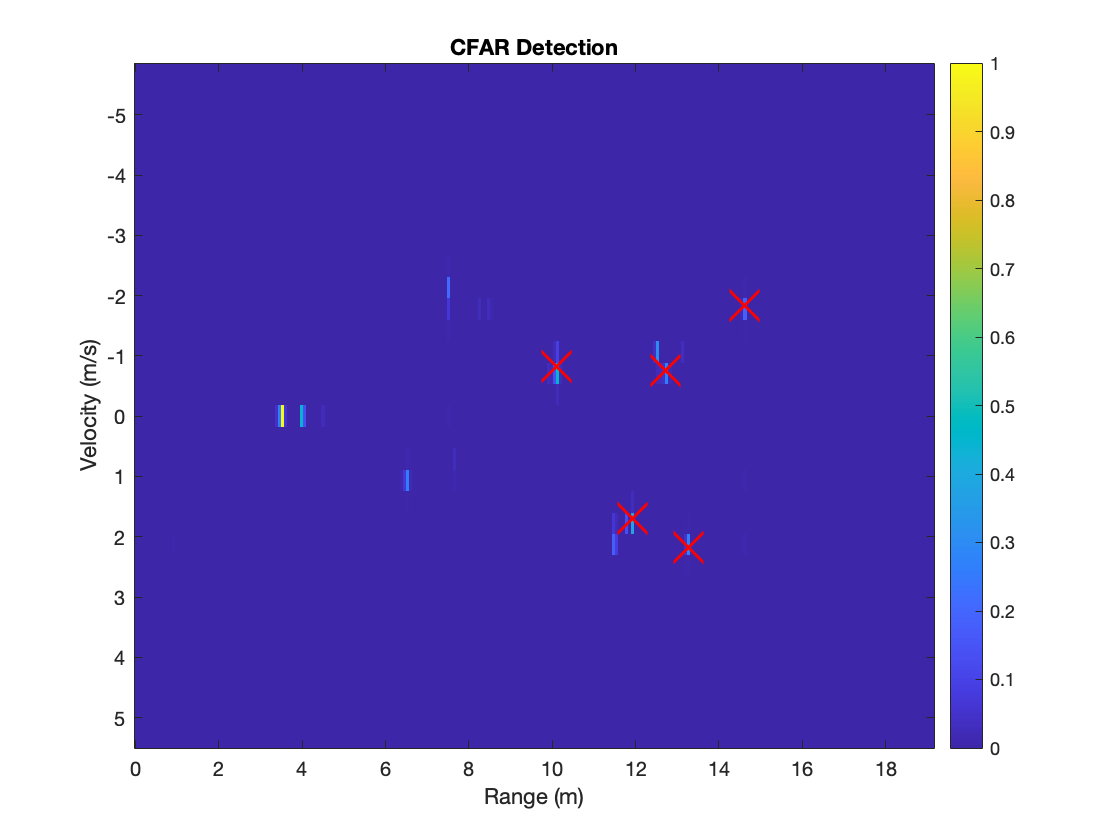
\includegraphics[height=0.8\textwidth]{figures/1c_empty.png}
                    \caption{CFAR without radiation pattern}
                \end{minipage}
                \begin{minipage}{0.45\textwidth}
                    \centering
                    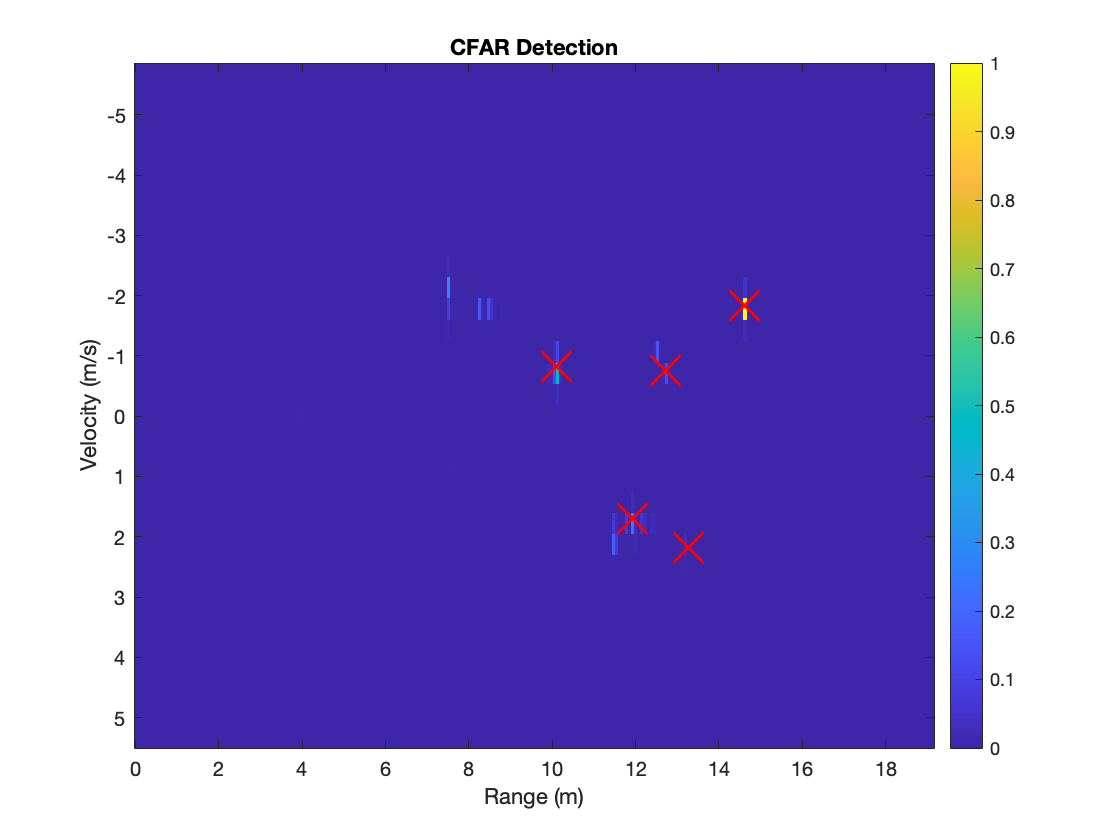
\includegraphics[height=0.8\textwidth]{figures/3c_beampattern.png}
                    \caption{CFAR with radiation pattern}
                \end{minipage}
            \end{figure}
	\end{itemize}
\end{frame}




\begin{frame}[t]{Results}
	\begin{itemize}
	    \item The view of the asymmetric radiation pattern in the room
        \vspace{1.0\baselineskip}
            \begin{figure}
            	\centering
            	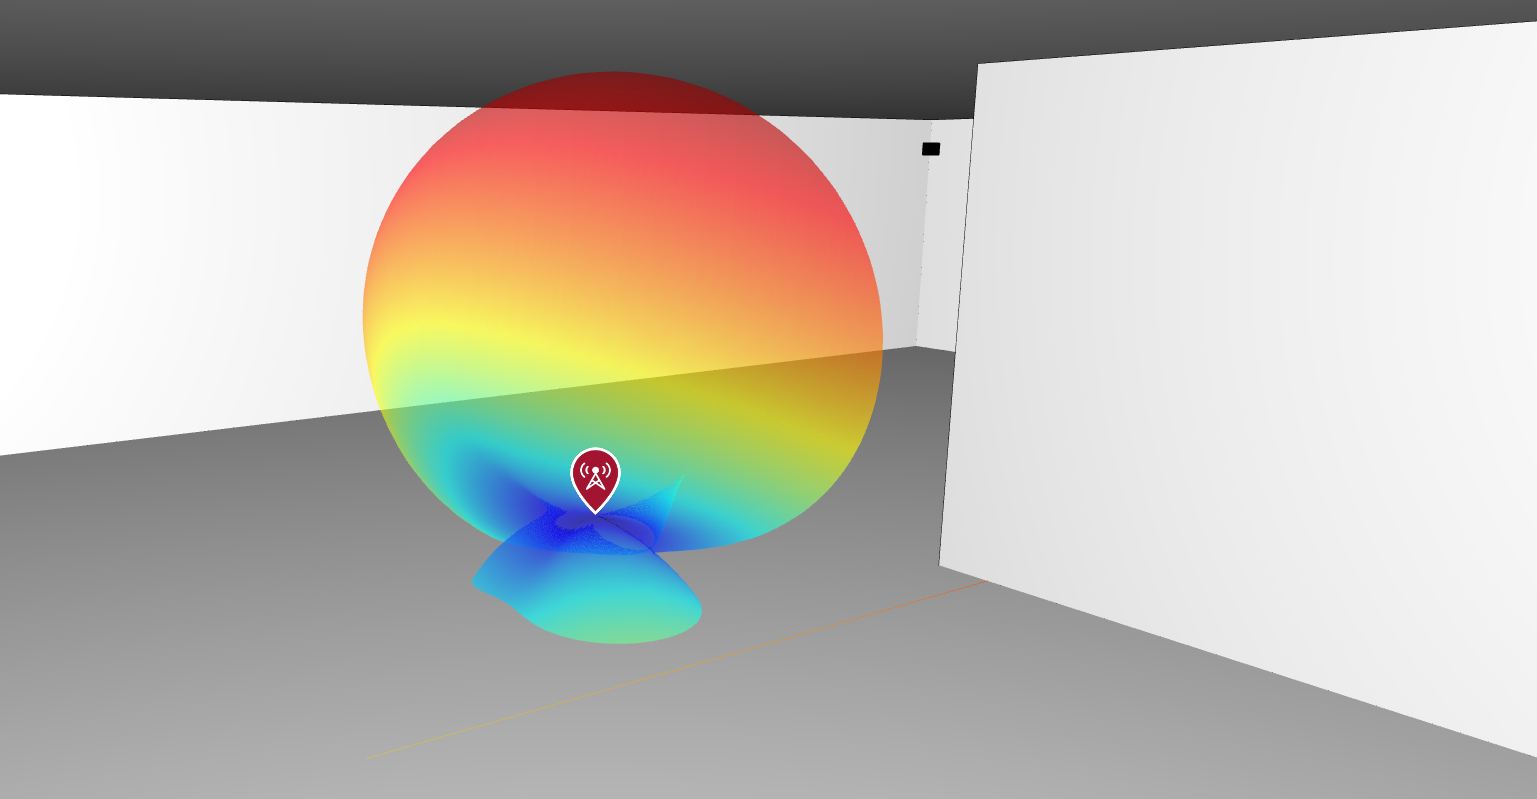
\includegraphics[scale=.17]{figures/asymmetric_antenna.png}
            	\caption{The view of the asymmetric pattern}
            \end{figure}
	\end{itemize}
\end{frame}


\section{Reflector radar cross section}
\subsection{Radar cross section}
\setcounter{section}{3}
\setcounter{figure}{0}
% -----------------------------------------------------------------------------
\begin{frame}[t]{Radar cross section (RCS)}
	\begin{itemize}
	    \item View of the RCS for the tetrahedral object with default parameters
        \vspace{0.5\baselineskip}
            \begin{figure}
                \centering
                \begin{minipage}{0.47\textwidth}
                    \centering
                    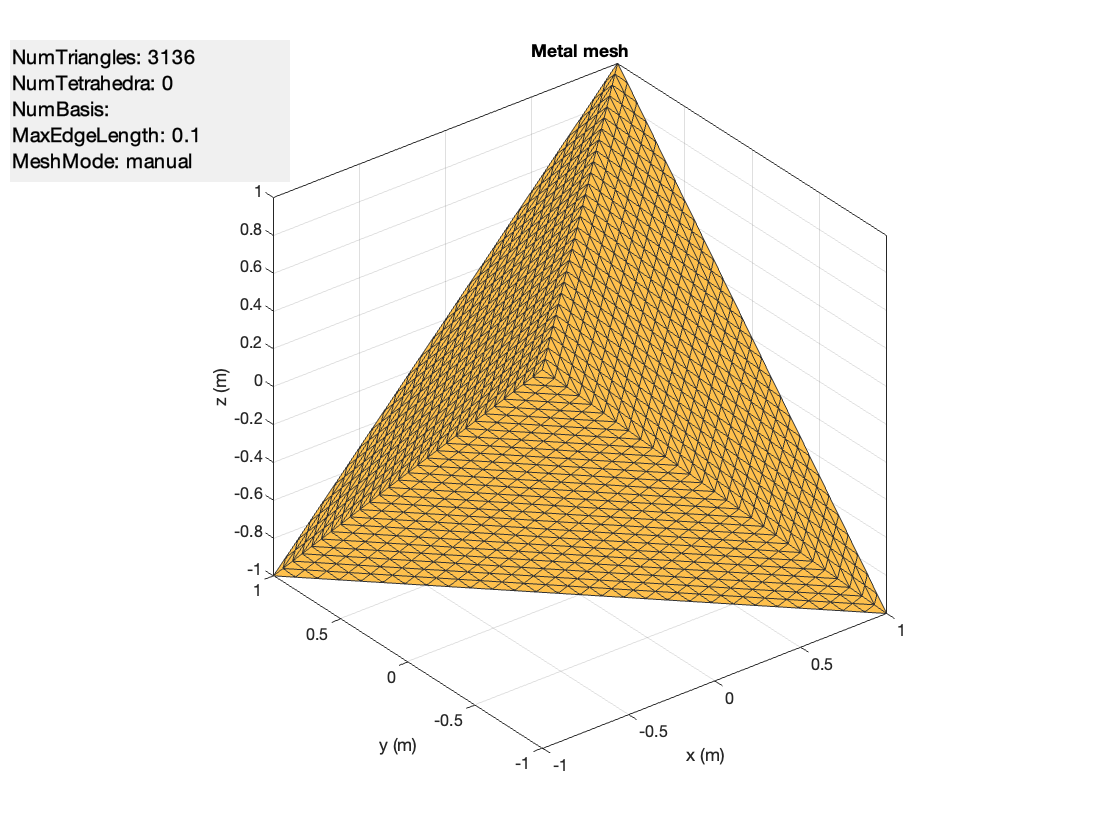
\includegraphics[height=0.7\textwidth]{figures/mesh_tetrahedral.png}
                    \caption{Mesh of the tetrahedral object}
                \end{minipage}
                \begin{minipage}{0.47\textwidth}
                    \centering
                    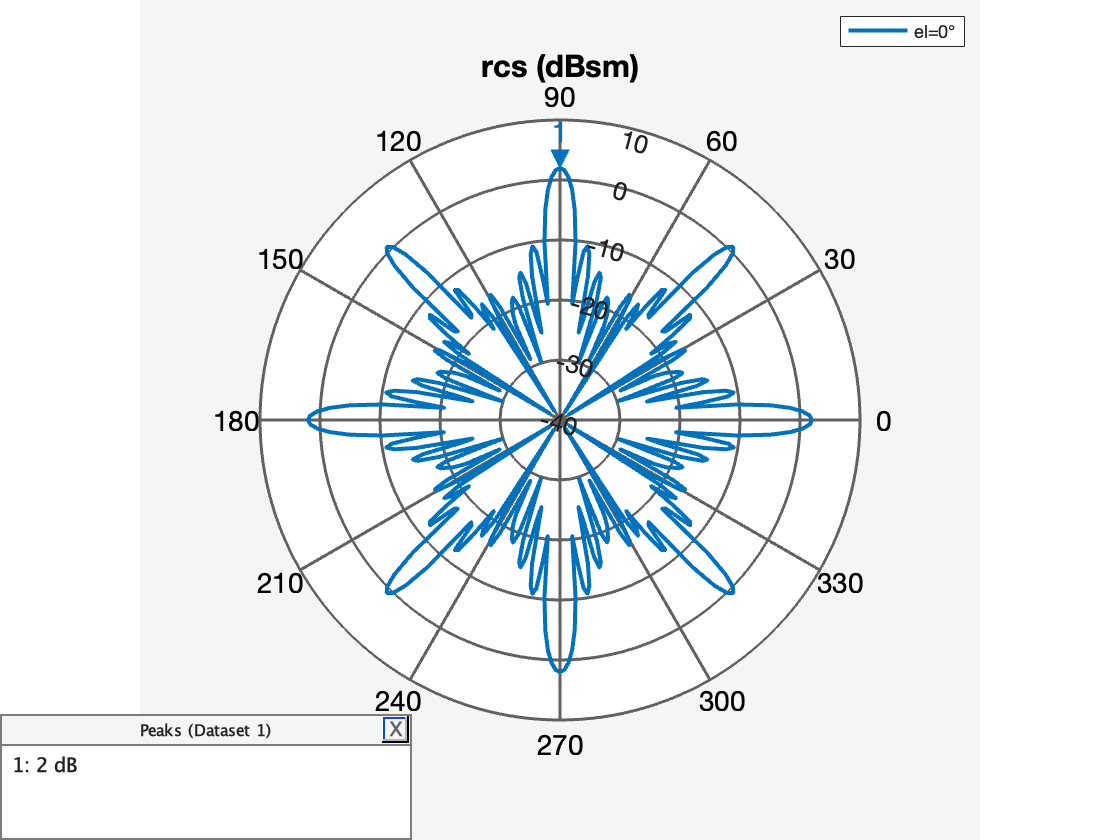
\includegraphics[height=0.7\textwidth]{figures/rcs_tetrahedral.png}
                    \caption{2D RCS of the tetrahedral object}
                \end{minipage}
            \end{figure}
	\end{itemize}
\end{frame}





\begin{frame}[t]{Radar cross section (RCS)}
	\begin{itemize}
	    \item View of the RCS for the tetrahedral object with scaled parameters
        \vspace{0.5\baselineskip}
            \begin{figure}
                \centering
                \begin{minipage}{0.47\textwidth}
                    \centering
                    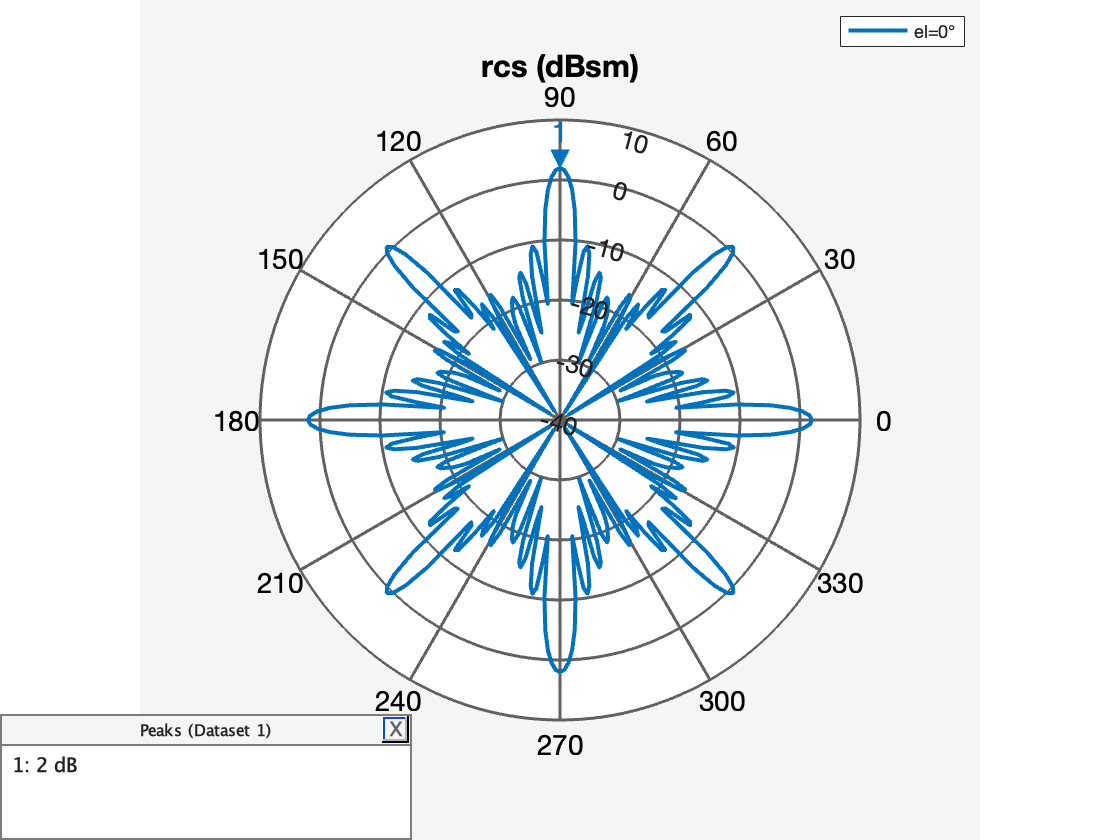
\includegraphics[height=0.7\textwidth]{figures/rcs_tetrahedral.png}
                    \caption{2D RCS without scaling}
                \end{minipage}
                \begin{minipage}{0.47\textwidth}
                    \centering
                    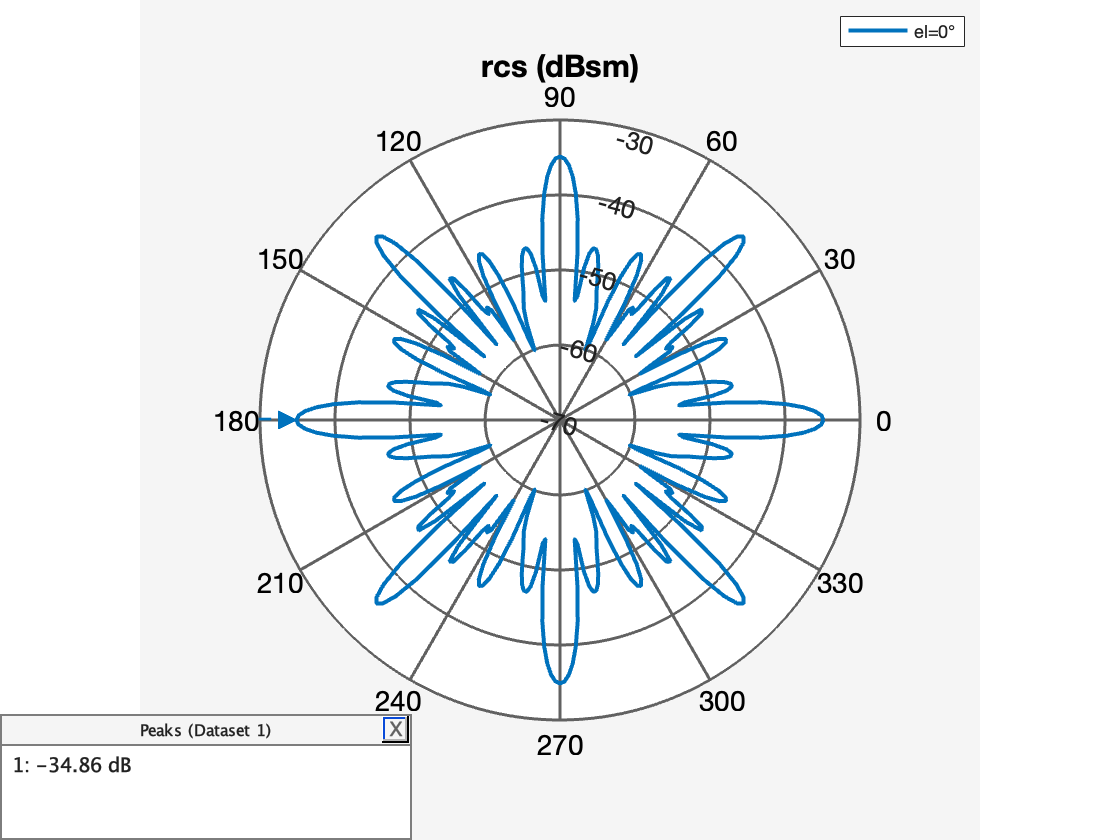
\includegraphics[height=0.7\textwidth]{figures/rcs_tetrahedral_scaled.png}
                    \caption{2D RCS with scaling}
                \end{minipage}
            \end{figure}
	\end{itemize}
\end{frame}





\begin{frame}[t]{Radar cross section (RCS)}
	\begin{itemize}
	    \item View of the RCS for the trihedral corner reflector
        \vspace{0.5\baselineskip}
            \begin{figure}
                \centering
                \begin{minipage}{0.47\textwidth}
                    \centering
                    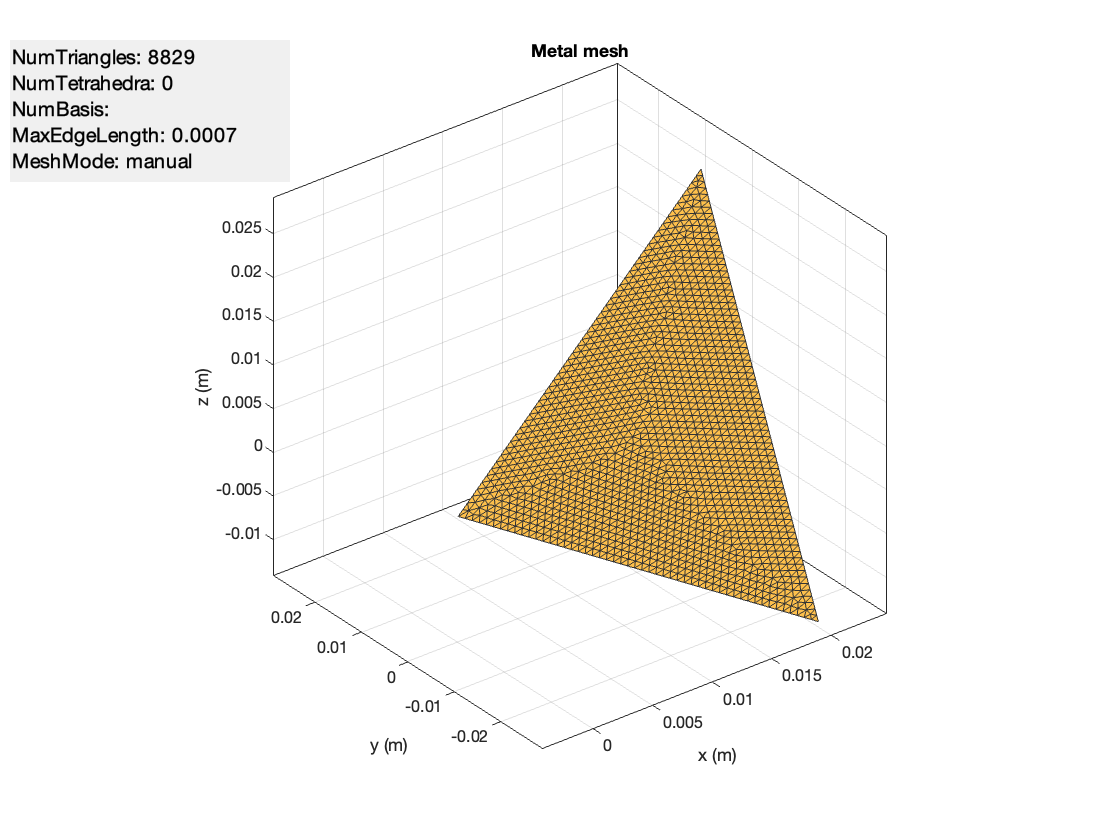
\includegraphics[height=0.7\textwidth]{figures/mesh_cr.png}
                    \caption{Mesh of trihedral corner reflector}
                \end{minipage}
                \begin{minipage}{0.47\textwidth}
                    \centering
                    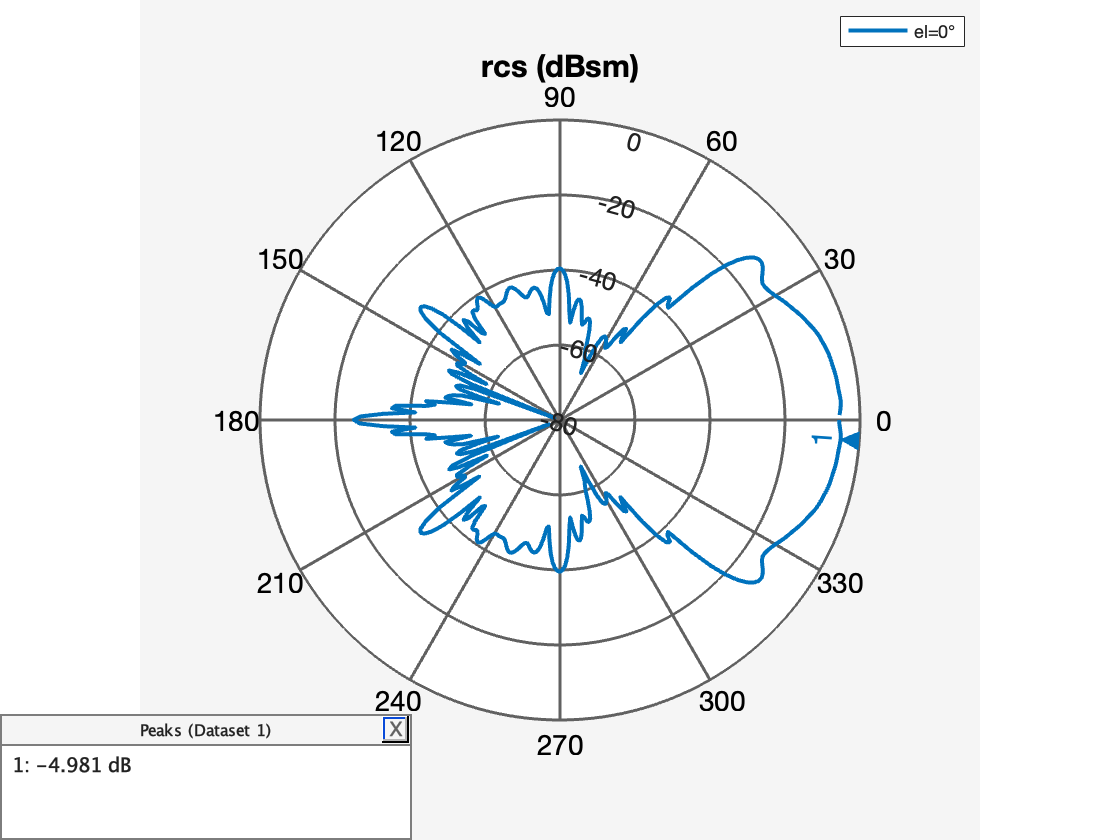
\includegraphics[height=0.7\textwidth]{figures/rcs_cr.png}
                    \caption{2D RCS of trihedral reflector}
                \end{minipage}
            \end{figure}
	\end{itemize}
\end{frame}




\begin{frame}[t]{Radar cross section (RCS)}
	\begin{itemize}
	    \item 3D RCS views for both reflectors
        \vspace{0.5\baselineskip}
            \begin{figure}
                \centering
                \begin{minipage}{0.47\textwidth}
                    \centering
                    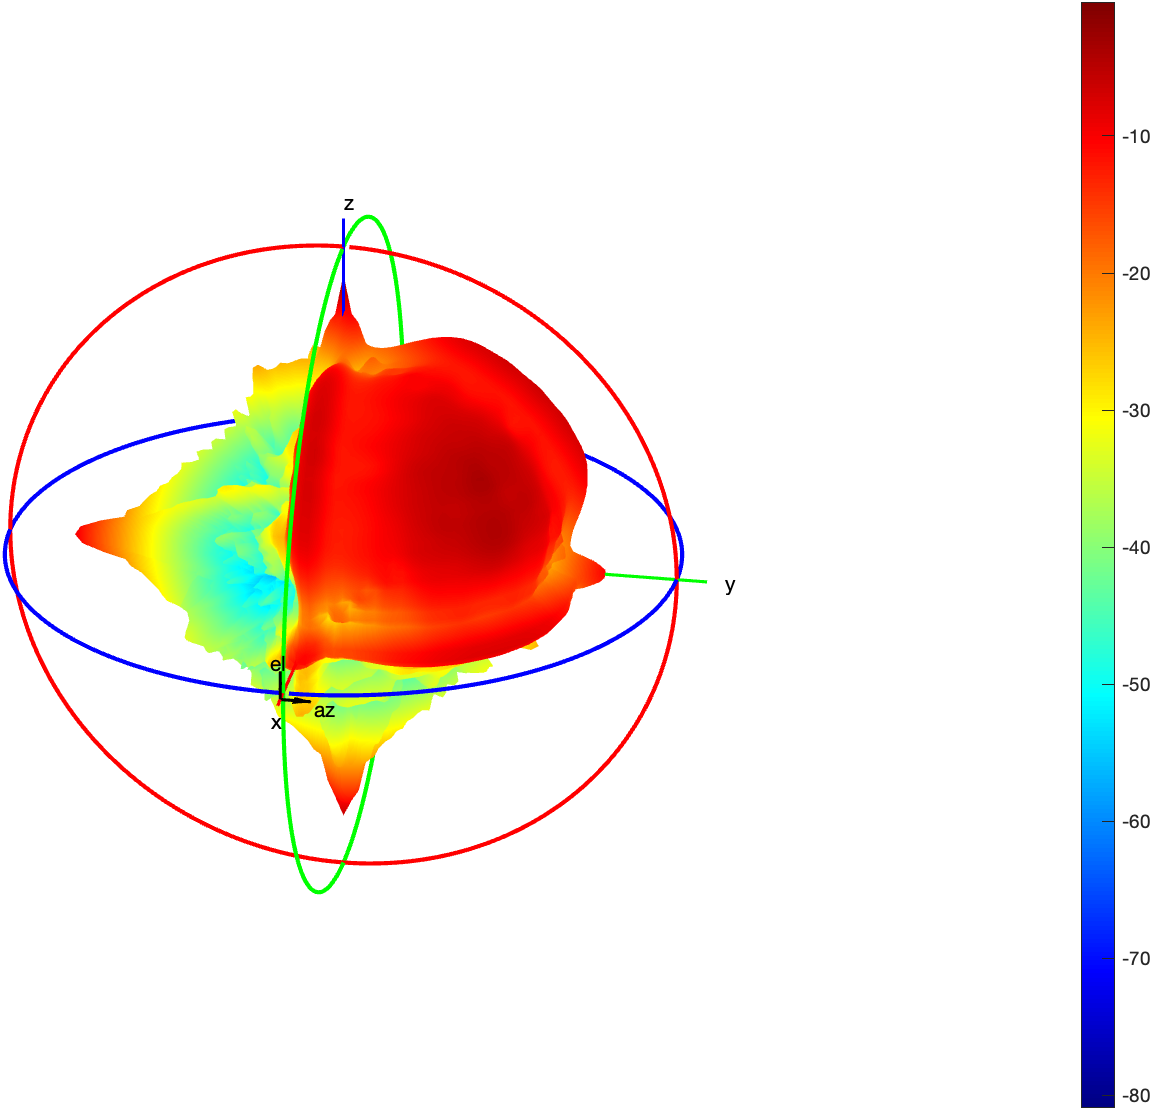
\includegraphics[height=0.7\textwidth]{figures/trihe_3d_rcs.png}
                    \caption{3D RCS of trihedral reflector}
                \end{minipage}
                \begin{minipage}{0.47\textwidth}
                    \centering
                    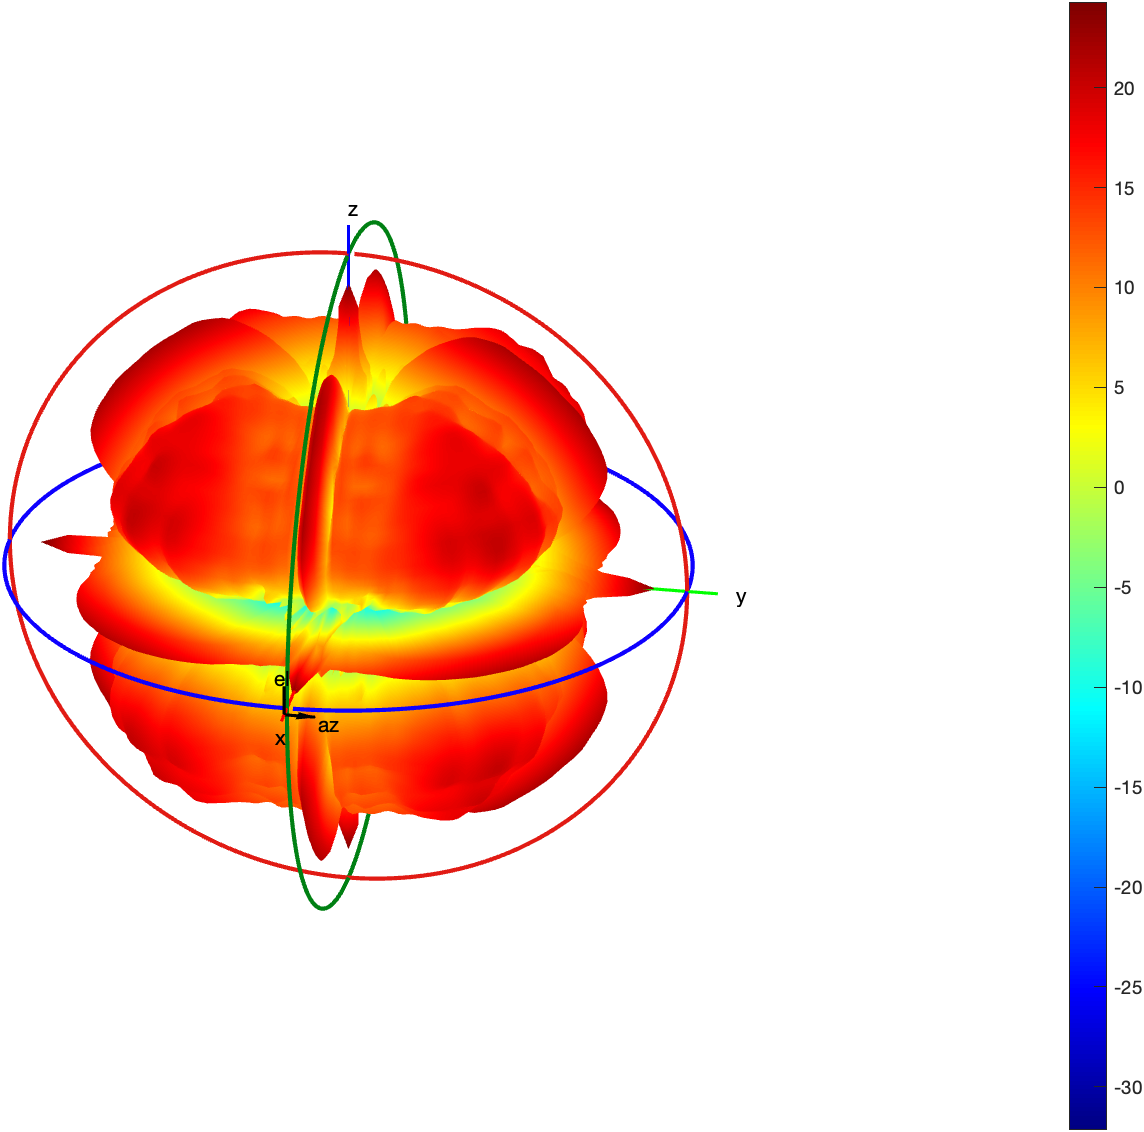
\includegraphics[height=0.7\textwidth]{figures/octa_3d_rcs.png}
                    \caption{3D RCS of octahedral reflector}
                \end{minipage}
            \end{figure}
	\end{itemize}
\end{frame}





\subsection{Results}
% -----------------------------------------------------------------------------
\begin{frame}[t]{Results}
	\begin{itemize}
	    \item The CFAR plots about the RCS pattern
        \vspace{0.5\baselineskip}
            \begin{figure}
                \centering
                \begin{minipage}{0.45\textwidth}
                    \centering
                    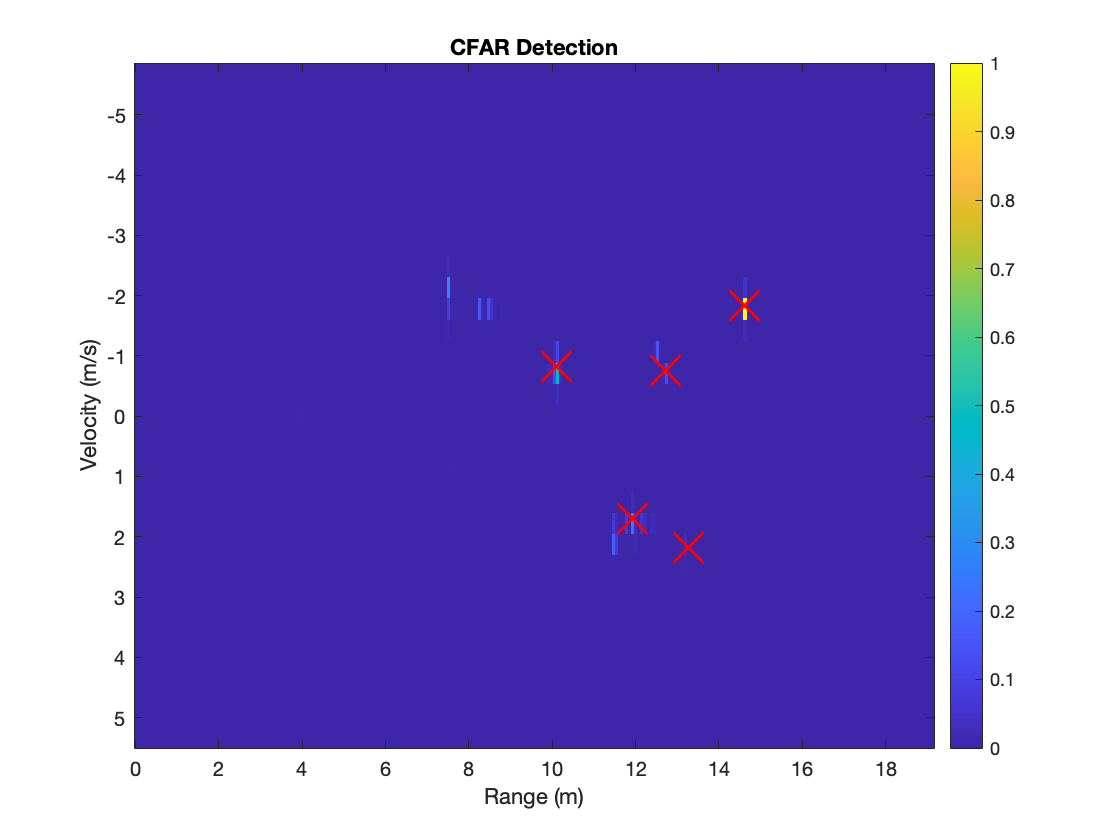
\includegraphics[height=0.8\textwidth]{figures/3c_beampattern.png}
                    \caption{With isotropic RCS pattern}
                \end{minipage}
                \begin{minipage}{0.45\textwidth}
                    \centering
                    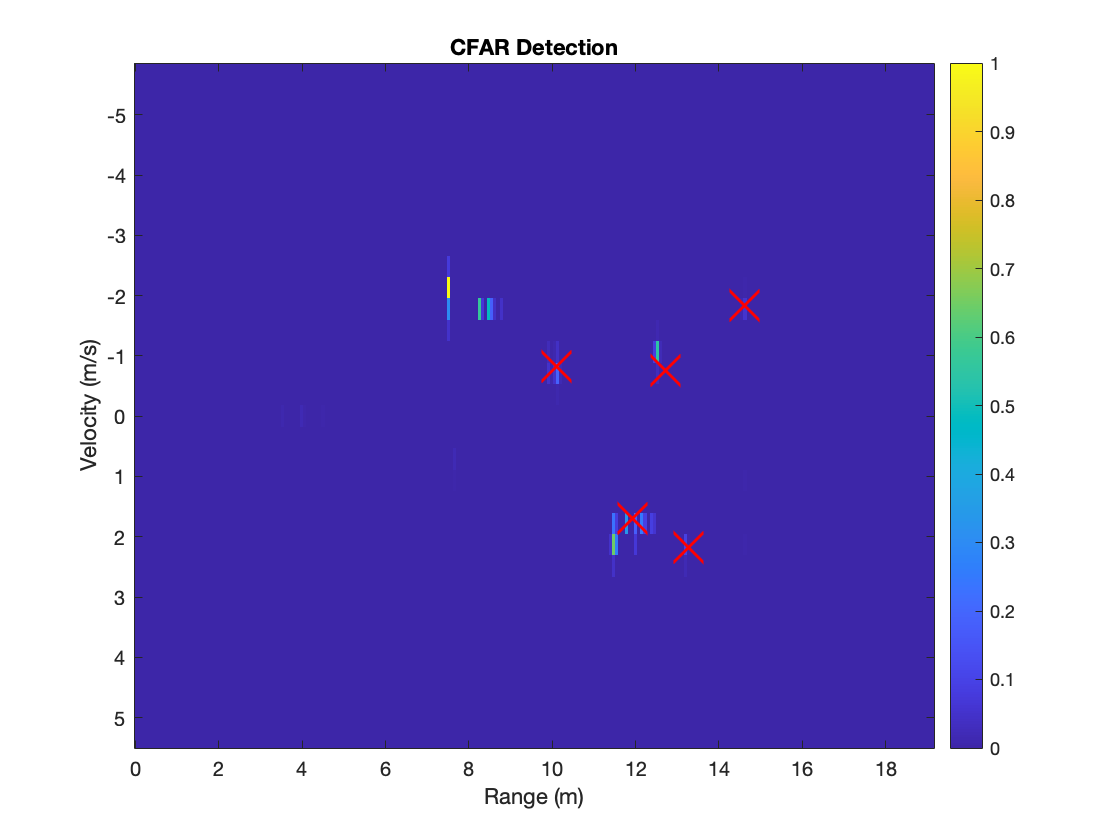
\includegraphics[height=0.8\textwidth]{figures/4c_empty.png}
                    \caption{With anisotropic RCS pattern}
                \end{minipage}
            \end{figure}
	\end{itemize}
\end{frame}




\section{Motion of the robot}
\subsection{Trajectory generation}
\setcounter{section}{4}
\setcounter{figure}{0}
% -----------------------------------------------------------------------------
\begin{frame}[t]{Trajectory generation}
	\begin{itemize}
	    \item The trajectory generation for the robot along the wall and furniture
        \vspace{0.5\baselineskip}
            \begin{figure}
            	\centering
            	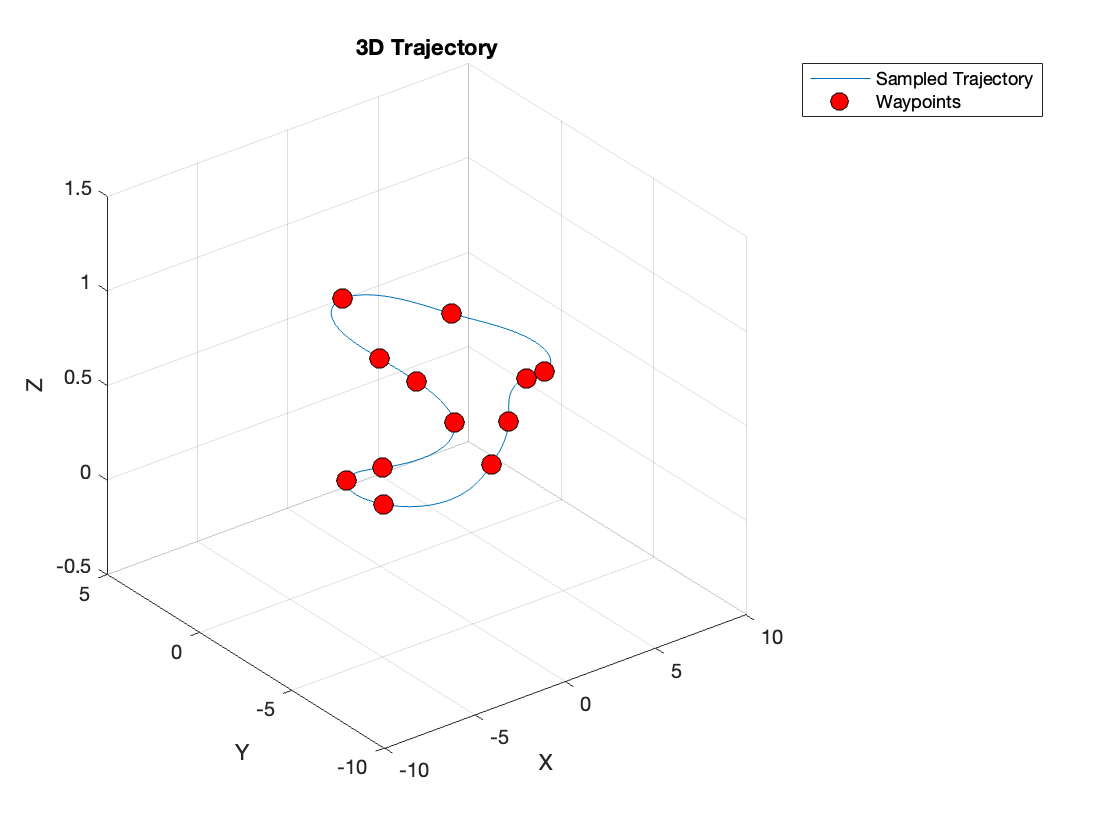
\includegraphics[scale=.18]{figures/trajectory.png}
            	\caption{The trajectory of the robot}
            \end{figure}
	\end{itemize}
\end{frame}





\subsection{Orientation}
% -----------------------------------------------------------------------------
\begin{frame}[t]{Orientation}
	\begin{itemize}
	    \item The orientation of the antenna during motion
        \vspace{1.0\baselineskip}
            \begin{figure}
                \centering
                \begin{minipage}{0.47\textwidth}
                    \centering
                    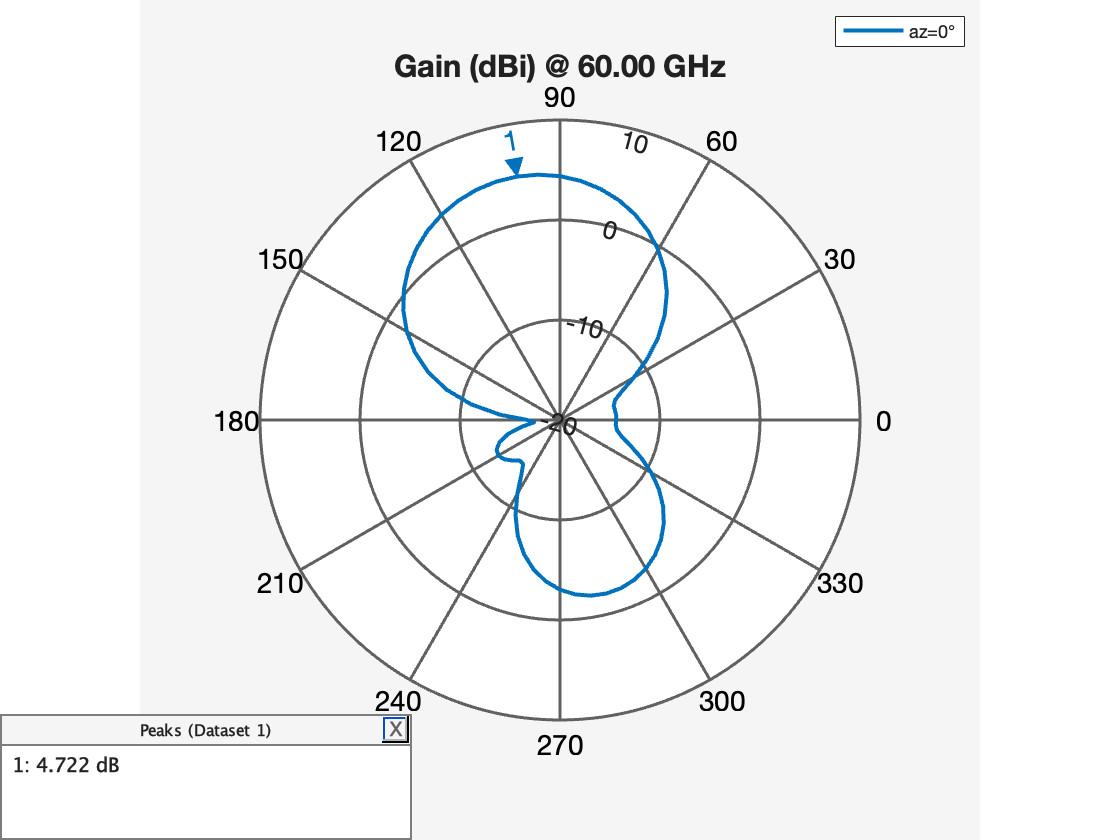
\includegraphics[height=0.7\textwidth]{figures/original_pattern.png}
                    \caption{Radiation pattern before rotation}
                \end{minipage}
                \begin{minipage}{0.47\textwidth}
                    \centering
                    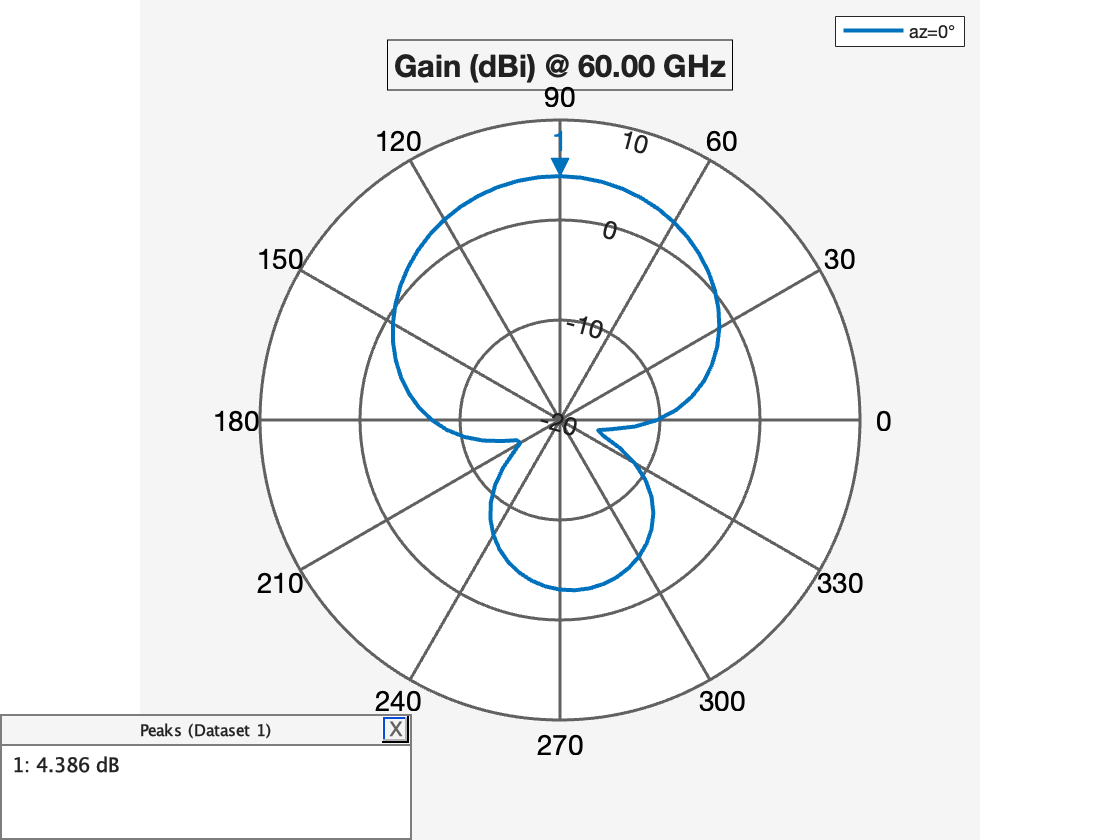
\includegraphics[height=0.7\textwidth]{figures/orientated_pattern.png}
                    \caption{Radiation pattern after rotation}
                \end{minipage}
            \end{figure}
	\end{itemize}
\end{frame}





\section{Evaluation}
\setcounter{section}{5}
\setcounter{figure}{0}
% -----------------------------------------------------------------------------

\begin{frame}[t]{Evaluation}
	\begin{itemize}
	    \item The CFAR plots difference in units watt (W) and decibel watt (dBW)
        \vspace{0.5\baselineskip}
            \begin{figure}
                \centering
                \begin{minipage}{0.45\textwidth}
                    \centering
                    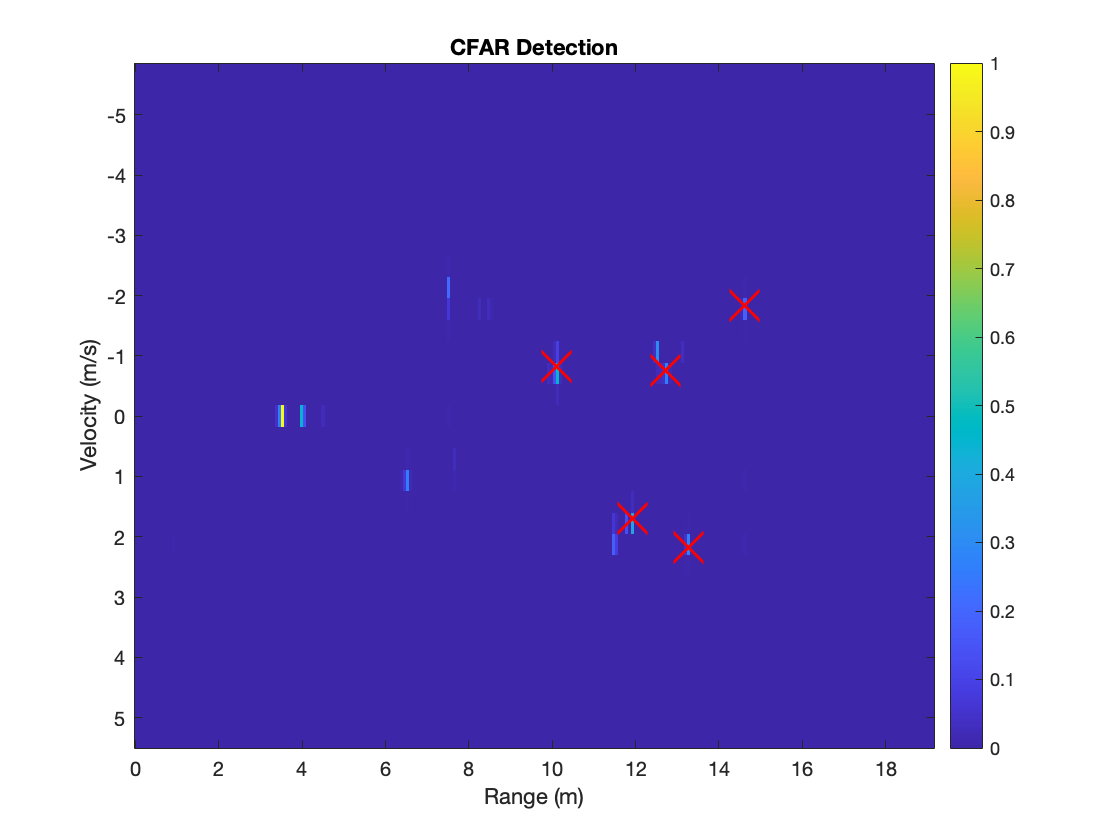
\includegraphics[height=0.8\textwidth]{figures/1c_empty.png}
                    \caption{CFAR plot in unit W}
                \end{minipage}
                \begin{minipage}{0.45\textwidth}
                    \centering
                    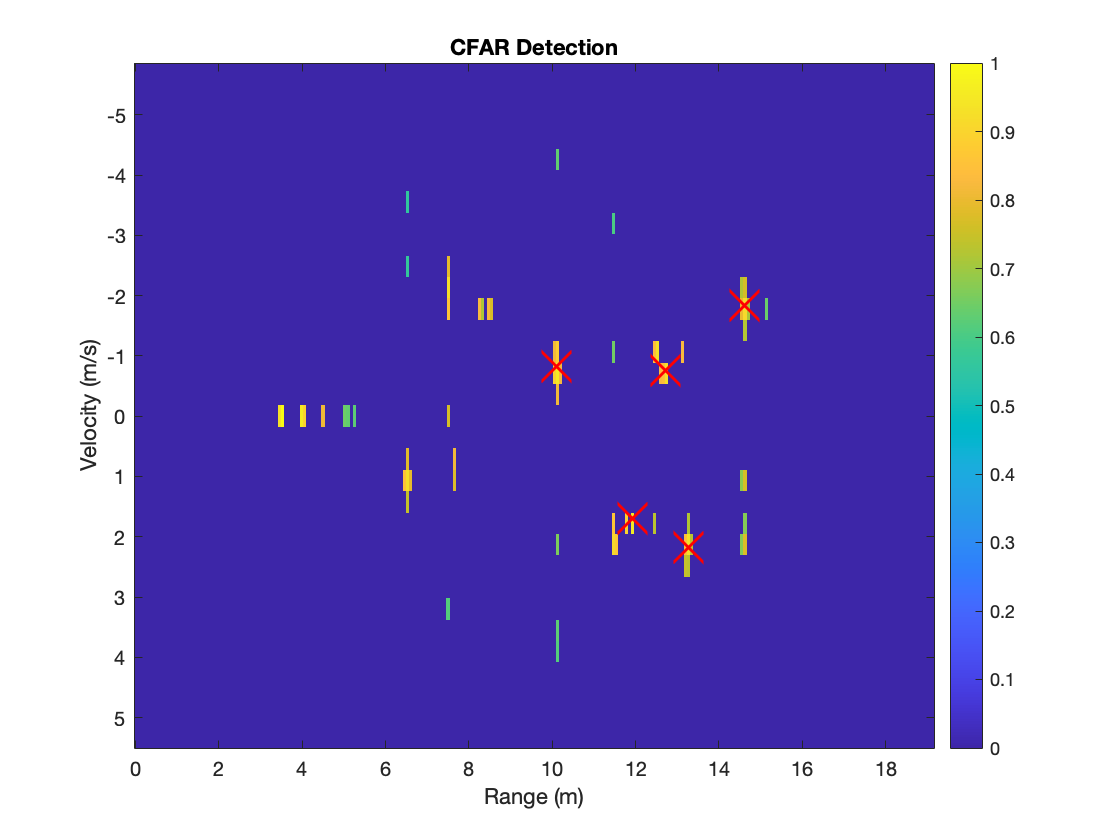
\includegraphics[height=0.8\textwidth]{figures/1c_empty_dBW.png}
                    \caption{CFAR plot in unit dBW}
                \end{minipage}
            \end{figure}
	\end{itemize}
\end{frame}





\begin{frame}[t]{Evaluation}
	\begin{itemize}
	    \item The CFAR plots with various positions and amount of reflectors in unit W
        \vspace{0.5\baselineskip}
            \begin{figure}
                \centering
                \begin{minipage}{0.45\textwidth}
                    \centering
                    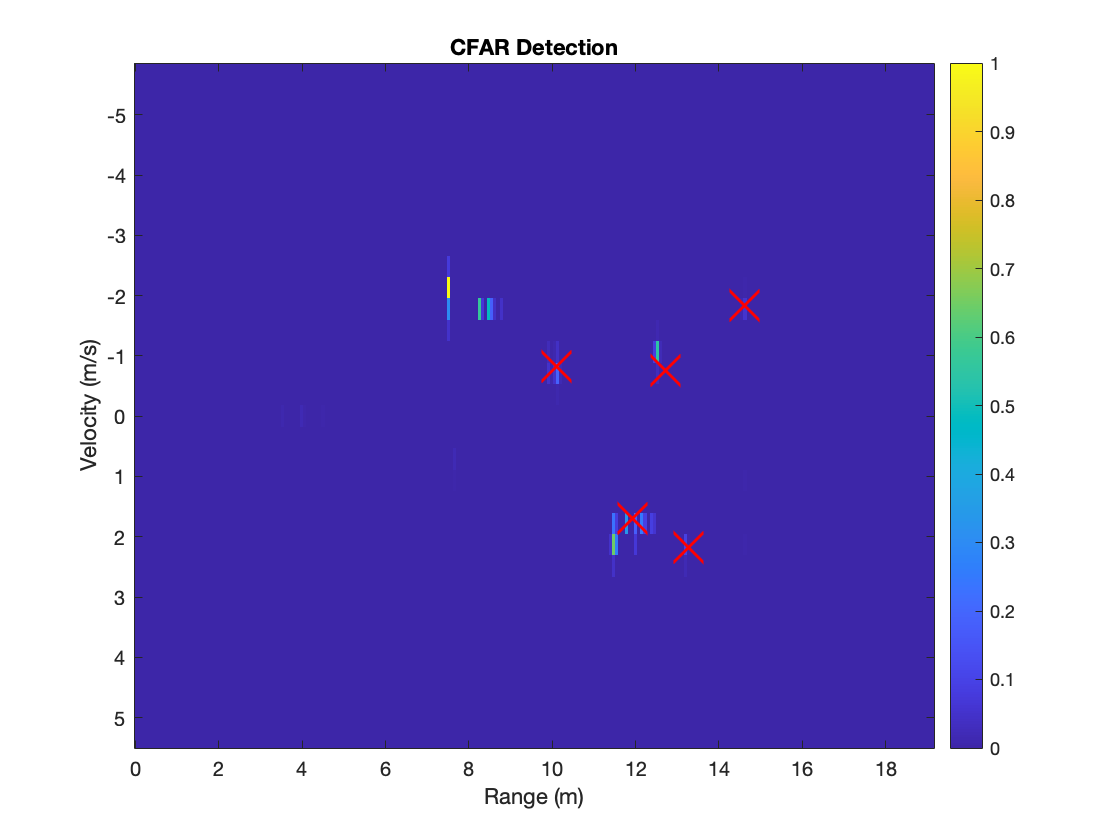
\includegraphics[height=0.8\textwidth]{figures/4c_empty.png}
                    \caption{CFAR plots with five trihedral corner reflectors}
                \end{minipage}
                \begin{minipage}{0.45\textwidth}
                    \centering
                    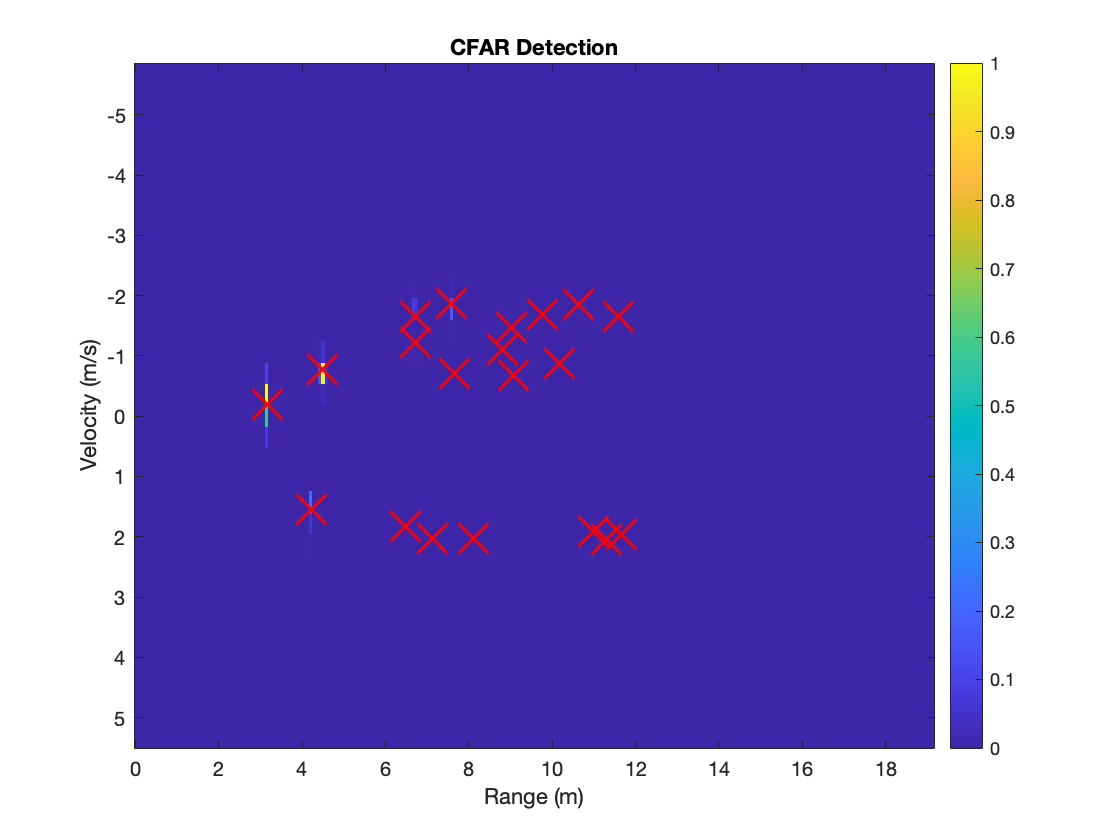
\includegraphics[height=0.8\textwidth]{figures/5c_octahedral.png}
                    \caption{CFAR plots with multiple octahedral reflectors}
                \end{minipage}
            \end{figure}
	\end{itemize}
\end{frame}





\begin{frame}[t]{Evaluation}
	\begin{itemize}
	    \item The meaning of the unit in the case of the multiple reflectors
        \vspace{0.5\baselineskip}
            \begin{figure}
                \centering
                \begin{minipage}{0.45\textwidth}
                    \centering
                    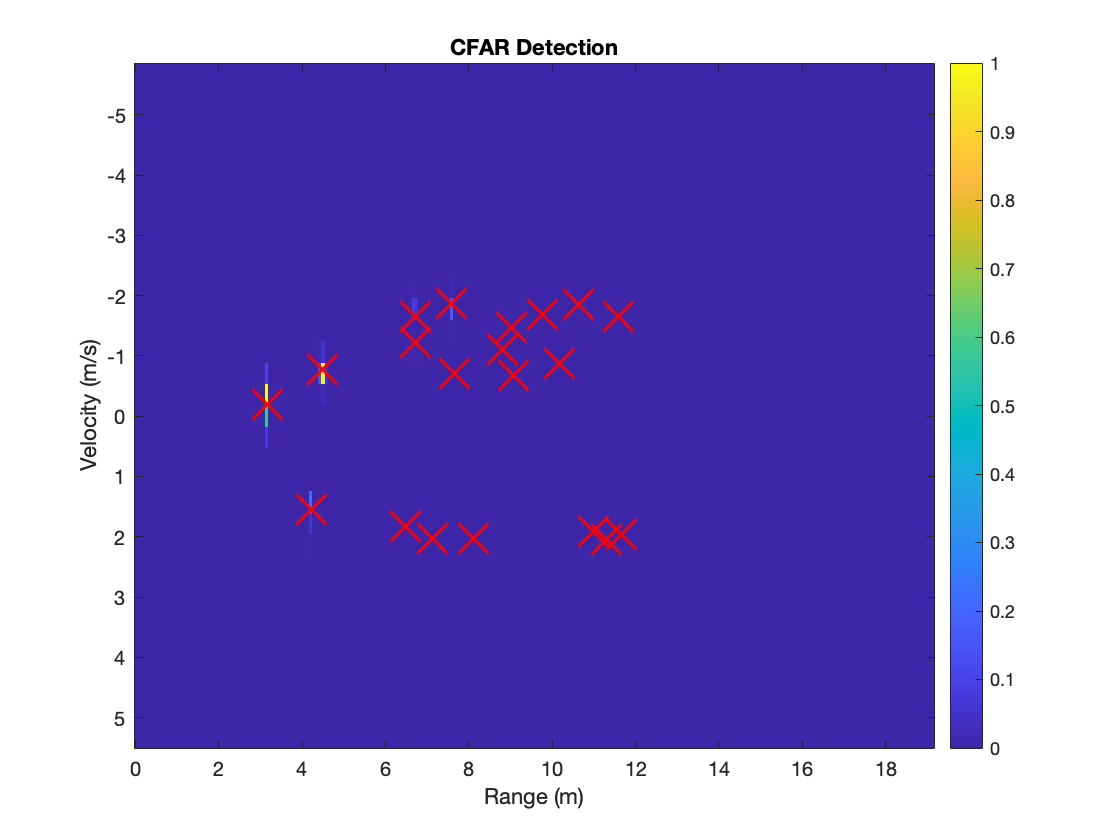
\includegraphics[height=0.8\textwidth]{figures/5c_octahedral.png}
                    \caption{CFAR plots in the unit W}
                \end{minipage}
                \begin{minipage}{0.45\textwidth}
                    \centering
                    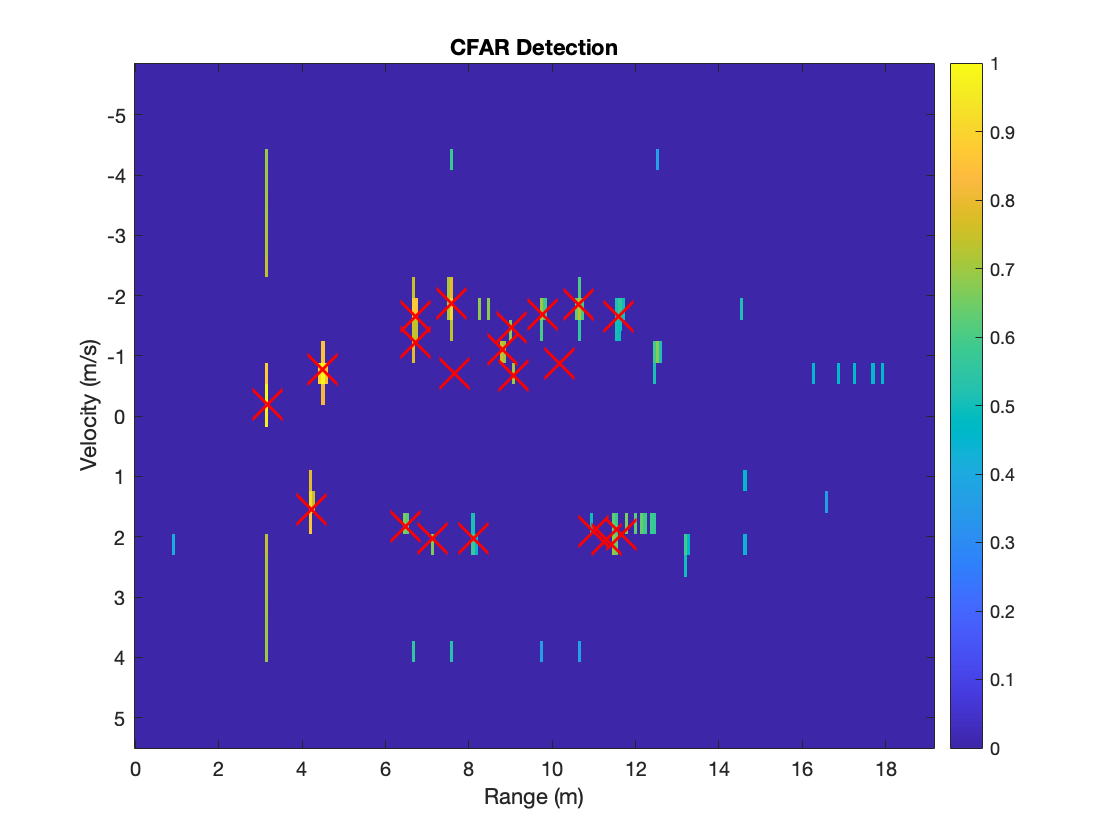
\includegraphics[height=0.8\textwidth]{figures/5c_octahedral_dBW.png}
                    \caption{CFAR plots in the unit dBW}
                \end{minipage}
            \end{figure}
	\end{itemize}
\end{frame}





% \begin{frame}[t]{Evaluation}
% 	\begin{itemize}
% 	    \item The CFAR plots with different maximum number of reflections
%         \vspace{0.5\baselineskip}
%             \begin{figure}
%                 \centering
%                 \begin{minipage}{0.45\textwidth}
%                     \centering
%                     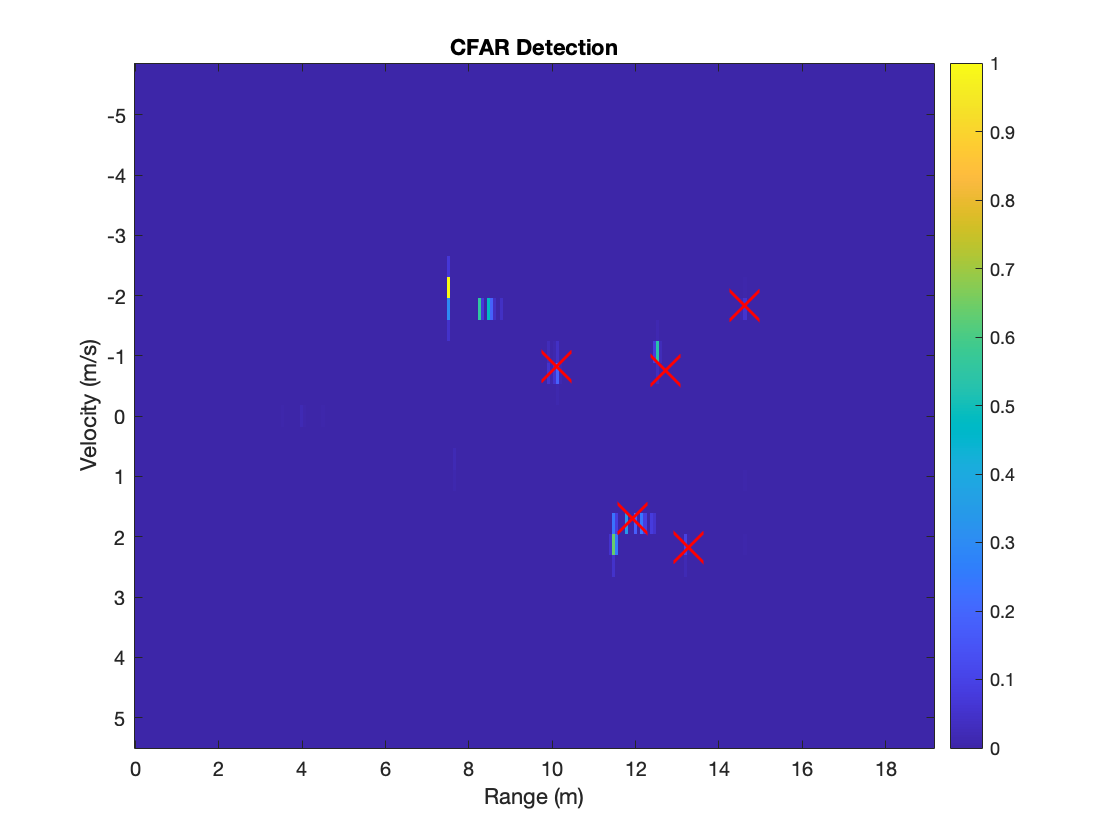
\includegraphics[height=0.8\textwidth]{figures/4c_rcs.png}
%                     \caption{Max four reflections}
%                 \end{minipage}
%                 \begin{minipage}{0.45\textwidth}
%                     \centering
%                     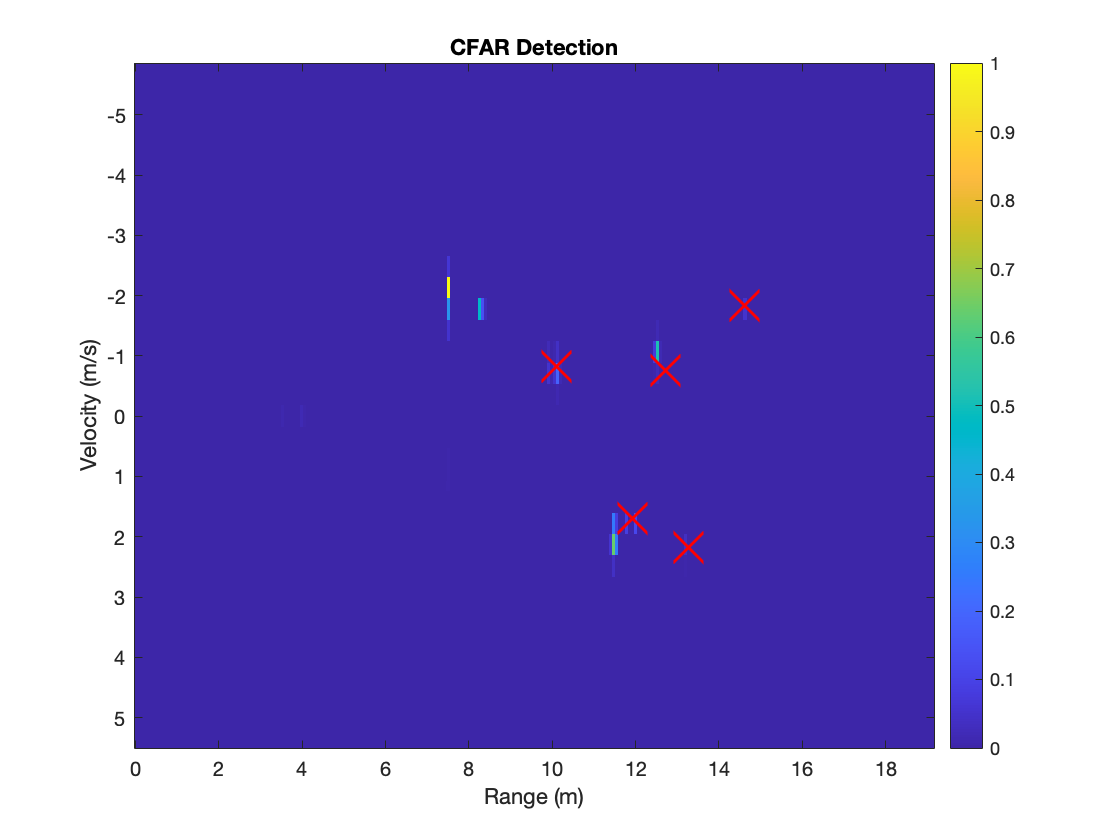
\includegraphics[height=0.8\textwidth]{figures/8c_reflection.png}
%                     \caption{Max two reflections}
%                 \end{minipage}
%             \end{figure}
% 	\end{itemize}
% \end{frame}




\begin{frame}[t]{Evaluation}
	\begin{itemize}
	    \item The CFAR plots along the trajectory generated in GIF format
        \vspace{0.5\baselineskip}
	\end{itemize}
    \centering
    \begin{figure}
        \centering
        \animategraphics[width=0.5\linewidth, autoplay=True]{2}{cfar_png/}{1}{54}
        \caption{CFAR plots along the trajectory}
    \end{figure}
\end{frame}




\section{Summary and outlook}
% -----------------------------------------------------------------------------
\begin{frame}[t]{Summary and outlook}
	\begin{itemize}
	    \item Summary: The ray tracing channel model works well and meets the goal.
        \vspace{0.5\baselineskip}
        \item Outlook:
        \vspace{0.5\baselineskip}
        \begin{itemize}
            \item Ray tracing with the surface diffraction
            \vspace{0.5\baselineskip}
            \item Antenna designer
            \vspace{0.5\baselineskip}
            \item RCS pattern simulation without scaling
            \vspace{0.5\baselineskip}
            \item Parallelizable computation of the simulation on GPU
            \vspace{0.5\baselineskip}
            \item Optimization of the number and arrangement of the reflectors
            \vspace{0.5\baselineskip}
            \item Combining with the deep learning for indoor localization system
        \end{itemize}
        
	\end{itemize}
\end{frame}



% -----------------------------------------------------------------------------
% Reference slide
\renewcommand*{\bibfont}{\scriptsize}
\begin{frame}[t]{Reference}
	\ifthenelse{\equal{\doclang}{german}}{
    	\bibliographystyle{IEEEtran_ISSger}
    }{
    	\bibliographystyle{IEEEtran_ISS}
    }
    \printbibliography{}
\end{frame}




% -----------------------------------------------------------------------------
\begin{frame}[t]
    \centering
    \fontsize{30}{120}\selectfont
	\textbf{Thank you for your attention}
\end{frame}

% -----------------------------------------------------------------------------


\end{document}
